\documentclass[lettersize,journal]{IEEEtran}
\usepackage{amsmath,amsfonts}
\usepackage{algorithmic}
\usepackage{algorithm}
\usepackage{array}
\usepackage[caption=false,font=normalsize,labelfont=sf,textfont=sf]{subfig}
\usepackage{textcomp}
\usepackage{stfloats}
\usepackage{url}
\usepackage{verbatim}
\usepackage{graphicx}
\usepackage{cite}
\usepackage{bm}
\usepackage{float}
\usepackage[center]{caption}
% \hyphenation{op-tical net-works semi-conduc-tor IEEE-Xplore}

\begin{document}

\title{Aircraft Pitch Control via Static and Reinforcement Learning-Based Adaptive PID Controllers}

\author{Muhammad Alfiyandy Hariansyah (ID: 21023691),~\IEEEmembership{PhD Student,~HKUST}% <-this % stops a space
\thanks{This report is part of the final project of MECH-6910T, HKUST.}% <-this % stops a space
\thanks{Manuscript received December 15, 2024}}

% The paper headers
\markboth{MECH6910T - Project Final Report, December~2024}%
{Hariansyah \MakeLowercase{\textit{et al.}}: Aircraft Pitch Control via Static and Reinforcement Learning-Based Adaptive PID Controllers}

\maketitle

\begin{abstract}
In this project, a static Proportional-Integral-Derivative (PID) controller and a Reinforcement Learning (RL)-based adaptive PID controller are developed to control the pitch of an aircraft system. The static PID represents a traditional method where the PID gains are constant and tuned beforehand, while the RL-based adaptive PID represents an intelligent method where the PID gains are varying over time. The project begins with deriving the non-linear dynamic system from the first principles. Subsequently, the system of equations is linearized and separated into two uncoupled motions: longitudinal and lateral. The pitch controllers are then designed based on the linearized longitudinal equations. The aircraft considered here is a Cessna-172 due to the availability of its stability derivatives. This report presents and discusses results for both static PID- and RL-based adaptive PID-controlled pitch simulations.
\end{abstract}

\begin{IEEEkeywords}
Aircraft pitch control, PID, adaptive tuning, reinforcement learning, linearization, Cessna-172
\end{IEEEkeywords}

\section{Introduction}

\IEEEPARstart{I}{n} aviation, precise control over an aircraft’s attitude is critical for ensuring stability, responsiveness, and safety during flight operations. The motion of an aircraft is highly complicated, coupled, and non-linear \cite{ref1}, described via a 6-DOF motion: three translational motions (vertical, horizontal, transverse) and three rotational motions (roll, pitch, yaw). The control over these motions is achieved by regulating the throttle and the control surfaces: elevator, aileron, and rudder. Furthermore, the control system is separated for two uncoupled motions: longitudinal and lateral. The longitudinal motion describes the pitch and velocity attitudes controlled by the throttle and elevator. Meanwhile, the lateral motion describes the roll and yaw attitudes, controlled by aileron and rudder.

Controlling the pitch of an aircraft in longitudinal motion can be achieved by regulating the elevator and keeping the constant thrust. To reduce the complexity, the aircraft is assumed to have a rigid body, and its motion is only a small deviation from its equilibrium flight condition \cite{ref2}, i.e., level unaccelerated flight. In this way, the highly coupled and non-linear system of equations can be linearized and used to design our controllers. Although, recent works have developed the flexibility part in the aircraft modeling \cite{ref3}.

Aircraft pitch control is not a new problem. Others have developed pitch controllers based on traditional methods, such as Proportional-Integral-Derivative (PID) \cite{ref4}, Linear-Quadratic-Regulator (LQR) \cite{ref5}, and Observer-State-Feedback (OSF) \cite{ref6}. These methods rely on static gains that are tuned and optimized beforehand. However, they possess a strong static performance in a single condition they are tuned for, and their performance is reduced when exposed to time-varying uncertain factors \cite{ref7}. Recent works have also attempted to use intelligent methods, such as a Fuzzy PID \cite{ref8}, Back-Propagation Neural Network \cite{ref9}, and Reinforcement Learning (RL) \cite{ref7,ref10}, which have some self-tuning and self-optimization features of the control parameters. Tuning of control parameters can be achieved via manual tuning, optimization, or RL. Mohanty et al. \cite{ref7}, for example, uses a class of RL algorithm called Deep Deterministic Policy Gradient (DDPG) \cite{ref11} to tune the PID controller.

Although aircraft pitch control has been extensively studied, there still remains an open challenge both in the modeling and control parts. In this project, a highly coupled and non-linear system of equations is modeled, assuming aircraft data for Cessna-172 \cite{ref12}, see Appendix \ref{apdx:Cessna172-data}. Subsequently, linearization is performed to derive the linear equations. Finally, a traditional PID control with different static gains and an RL-based adaptive PID control with different neural network architectures under Proximal Policy Optimization (PPO) \cite{ref13} framework are compared and their performance is discussed.

\section{Non-linear coupled 6-DOF aircraft motion}
The equations of motion for a flight vehicle usually are written in a body-fixed coordinate system. The body velocities are defined as: $\overrightarrow{v}_{\mathrm{B}}=(u,v,w)^\mathrm{T}$, while body angular rates are defined as: $\overrightarrow{\Omega}_{\mathrm{B}}=(p,q,r)^\mathrm{T}$. The velocities can also be written in earth-fixed coordinate system ($xyz$-axis) as $\overrightarrow{v}_{\mathrm{E}}=(\dot{x},\dot{y},\dot{z})^\mathrm{T}$. In similar manner, the roll, pitch, and yaw angles are defined as $\phi$, $\theta$, and $\psi$, respectively. The following transformation can be done to relate the body velocities $\overrightarrow{v}_{\mathrm{B}}$ to $\overrightarrow{v}_{\mathrm{E}}$: $\overrightarrow{v}_{\mathrm{E}}=\mathcal{L}_{\mathrm{B}\rightarrow\mathrm{E}}\,\overrightarrow{v}_{\mathrm{B}}$, where $\mathcal{L}_{\mathrm{B}\rightarrow\mathrm{E}}$ is the body-to-earth transformation matrix, see Appendix \ref{apdx:EoM} for details. By performing body-to-earth transformation on velocities, the following equations are obtained:
\begin{equation}\label{eq:x_dot}
\dot{x}=u\,c\psi\,c\theta-v\,(c\phi\,s\psi-c\psi\,s\phi\,s\theta)+w\,(s\phi\,s\psi+c\phi\,c\psi\,s\theta)
\end{equation}
\begin{equation}\label{eq:y_dot}
\dot{y}=u\,c\theta\,s\psi+v\,(c\phi\,c\psi+s\phi\,s\psi\,s\theta)-w\,(c\psi\,s\phi-c\phi\,s\psi\,s\theta)
\end{equation}
\begin{equation}\label{eq:z_dot}
\dot{z}=-u\,s\theta+v\,c\theta\,s\phi+w\,c\phi\,c\theta
\end{equation}
where $s$ and $c$ correspond to the $sin$ and $cos$ of the angles. In similar manner, the body-to-earth transformation can also be applied to the angular rates, yielding the following equations:
\begin{equation}\label{eq:phi_dot}
\dot{\phi}=p+r\,\cos\phi\,\tan\theta+q\,\sin\phi\,\tan\theta
\end{equation}
\begin{equation}\label{eq:theta_dot}
\dot{\theta}=q\,\cos\phi-r\,\sin\phi
\end{equation}
\begin{equation}\label{eq:psi_dot}
\dot{\psi}=(r\,\cos\phi+q\,\sin\phi)/\cos\theta
\end{equation}

The force equation in translational motion in body-fixed frame is: $\overrightarrow{F}_{\mathrm{ext}}=m\,\left(\dot{\overrightarrow{v}_{\mathrm{B}}} + \overrightarrow{\Omega}_{\mathrm{B}} \times \overrightarrow{v}_{\mathrm{B}} \right)$. In similar manner, the moment equation in rotational motion in body-fixed frame is: $\overrightarrow{M}_{\mathrm{ext}}=I_{\mathrm{B}}\,\dot{\overrightarrow{\Omega}_{\mathrm{B}}} + \overrightarrow{\Omega}_{\mathrm{B}} \times \left(I_{\mathrm{B}}\,\overrightarrow{\Omega}_{\mathrm{B}}\right)$. The force $\overrightarrow{F}_{\mathrm{ext}}$ and the moment $\overrightarrow{M}_{\mathrm{ext}}$ are the resultant external force and moment from various sources: aerodynamics, propulsion, and gravity.

Expanding the force and moment equations in three translational and three rotational axes yield:
\begin{equation}\label{eq:f_ext_x}
F_{\mathrm{ext,x}}=m\,\left(\dot{u}+q\,w-r\,v\right)
\end{equation}
\begin{equation}\label{eq:f_ext_y}
F_{\mathrm{ext,y}}=m\,\left(\dot{v}-p\,w+r\,u\right)
\end{equation}
\begin{equation}\label{eq:f_ext_z}
F_{\mathrm{ext,z}}=m\,\left(\dot{w}+p\,v-q\,u\right)
\end{equation}
\begin{equation}\label{eq:m_ext_x}
M_{\mathrm{ext,x}}=I_{\mathrm{xx}}\,\dot{p}-I_{\mathrm{xz}}\,\dot{r}-q\,\left(I_{\mathrm{zx}}\,p-I_{\mathrm{zz}}\,r\right)-I_{\mathrm{yy}}\,q\,r
\end{equation}
\begin{equation}\label{eq:m_ext_y}
M_{\mathrm{ext,y}}=I_{\mathrm{yy}}\,\dot{q}+p\,\left(I_{\mathrm{zx}}\,p-I_{\mathrm{zz}}\,r\right)+r\,\left(I_{\mathrm{xx}}\,p-I_{\mathrm{xz}}\,r\right)
\end{equation}
\begin{equation}\label{eq:m_ext_z}
M_{\mathrm{ext,z}}=I_{\mathrm{zz}}\,\dot{r}-I_{\mathrm{zx}}\,\dot{p}-q\,\left(I_{\mathrm{xx}}\,p-I_{\mathrm{xz}}\,r\right)+I_{\mathrm{yy}}\,p\,q
\end{equation}
where $m$ is the mass of the aircraft, $\boldsymbol{I}$ is the aircraft moment of inertia. Equations (\ref{eq:f_ext_x}-\ref{eq:f_ext_z}) are used to solve for the translational acceleration in body-fixed frame: $\dot{\overrightarrow{v}_{\mathrm{B}}}=(\dot{u}, \dot{v}, \dot{w})^\mathrm{T}$, while Equations (\ref{eq:m_ext_x}-\ref{eq:m_ext_z}) are used to solve for the rotational acceleration in body-fixed frame: $\dot{\overrightarrow{\Omega}_{\mathrm{B}}}=(\dot{p}, \dot{q}, \dot{r})^\mathrm{T}$.

Finally, Equations (\ref{eq:x_dot}-\ref{eq:m_ext_z}) represent the non-linear, coupled, first order system of equations that describe the 6-DOF aircraft motion. The details of the derivation for each of the external forces $\overrightarrow{F}_{\mathrm{ext}}$ and moments $\overrightarrow{M}_{\mathrm{ext}}$ can be found in Appendix \ref{apdx:aero} for the aerodynamics and Appendix \ref{apdx:propulsion} for propulsion. The atmosphere is modeled using the International Standard Atmosphere (ISA) \cite{ref16}, see Appendix \ref{apdx:ISA} for the details.

\section{Aircraft pitch dynamic modeling}

\subsection{Trim condition}
Let's define a vector of motion states as:
\begin{equation}\label{eq:full_states}
\bm{x}=(x, y, z, \phi, \theta, \psi, p, q, r, u, v, w)^{\mathrm{T}}
\end{equation}
a vector of outputs as:
\begin{equation}\label{eq:full_outputs}
\bm{y}=(\bm{x},\alpha,\beta,\gamma,\zeta,v_{\mathrm{TAS}},\rho)^{\mathrm{T}}
\end{equation}
and a vector of control inputs as:
\begin{equation}\label{eq:full_states}
\bm{u}=(\delta_{\mathrm{e}}, \delta_{\mathrm{a}}, \delta_{\mathrm{r}}, \delta_{\mathrm{t}})^{\mathrm{T}}
\end{equation}
where $\delta_{\mathrm{e}}$, $\delta_{\mathrm{a}}$, and $\delta_{\mathrm{r}}$ are the deflection angles of elevator, aileron, and rudder, respectively, while $\delta_{\mathrm{t}}$ is the throttle input. Assume the aircraft is flying a level unaccelerated cruise at 5000 $ft$ (1524 $m$). The trim condition solves:
\begin{equation}\label{eq:trim_states}
\bm{x_\mathrm{0}}=(x_\mathrm{0}, y_\mathrm{0}, z_\mathrm{0}, \phi_\mathrm{0}, \theta_\mathrm{0}, \psi_\mathrm{0}, p_\mathrm{0}, q_\mathrm{0}, r_\mathrm{0}, u_\mathrm{0}, v_\mathrm{0}, w_\mathrm{0)}^{\mathrm{T}}
\end{equation}
\begin{equation}\label{eq:zero_states_dot}
\begin{aligned}
\bm{\dot{x}_\mathrm{0}}&=f(\bm{x_\mathrm{0}})=0
\end{aligned}
\end{equation}

By assuming all the values for Cessna 172 aircraft \cite{ref12}, the above equations are solved in Matlab. The following solutions are found for the trimmed states, control inputs, and outputs.
\begin{equation}\label{eq:trim_states_vals}
\bm{x_{\mathrm{0}}}=(0, 0, -1524, 0, 0, 0, 62.3866, 0, 0, 0, 0, 0)^{\mathrm{T}}
\end{equation}
\begin{equation}\label{eq:trim_input_vals}
\bm{u_{\mathrm{0}}}=(-0.0032115, 0, 0, 0.6792)^{\mathrm{T}}
\end{equation}
\begin{equation}\label{eq:trim_output_vals}
\bm{y_{\mathrm{0}}}=(\bm{x_{\mathrm{0}}}, 0, 0, 0, 0, 62.3866, 1.0557)^{\mathrm{T}}
\end{equation}

\subsection{Linearized equations}
Equations (\ref{eq:x_dot}-\ref{eq:m_ext_z}) are non-linear and coupled. So, they need to be linearized. Linearization procedure assumes a small deviation from the previously trimmed states, i.e., $\bm{x}=\bm{x}_0+\Delta \bm{x}$. Therefore, the control input will be an additional input from the trimmed inputs, i.e., $\bm{u}=\bm{u}_0+\Delta \bm{u}$. In similar manner, the outputs will be $\bm{y}=\bm{y}_0+\Delta \bm{y}$. The linearization procedure is performed in Matlab, again by assuming the values for Cessna 172 aircraft, the following linear equations are obtained.
\begin{equation}
\Delta \bm{\dot{x}} = A\,\Delta\bm{x} + B\,\Delta\bm{u}
\end{equation}
\begin{equation}
\Delta\bm{y} = C\,\Delta\bm{x} + D\,\Delta\bm{u}
\end{equation}
where matrices $A$, $B$, $C$, and $D$ are the state space representation of the linearized twelve states differential equations. The numerical values details are presented in Appendix \ref{apdx:long_dyn} and \ref{apdx:lat_dyn}.

Matrices $A$, $B$, $C$, and $D$ can be separated into two uncoupled equations: longitudinal and lateral. Since we focus on pitch control, only longitudinal equations are used to design our controller. In longitudinal motion, the states are reduced into six states, the control inputs are reduced into two, and the outputs into ten:
\begin{equation}\label{eq:long_states}
\Delta \bm{x}_{\mathrm{long}} = (\Delta x, \Delta z, \Delta \theta, \Delta u, \Delta w, \Delta q)^{\mathrm{T}}
\end{equation}
\begin{equation}
\Delta \bm{u}_{\mathrm{long}} = (\Delta \delta _{\mathrm{e}}, \Delta \delta _{\mathrm{t}})^{\mathrm{T}}
\end{equation}
\begin{equation}
\Delta y_{\mathrm{long}} = (\Delta \bm{x}_{\mathrm{long}}, \Delta \alpha, \Delta \gamma, \Delta v_{\mathrm{TAS}}, \Delta \rho)^{\mathrm{T}}
\end{equation}

The resulting state-space representation for longitudinal motion is then written:
\begin{equation}
\Delta \bm{\dot{x}_{\mathrm{long}}} = A_{\mathrm{long}}\,\Delta\bm{x} + B_{\mathrm{long}}\,\Delta\bm{u}
\end{equation}
\begin{equation}
\Delta\bm{y_{\mathrm{long}}} = C_{\mathrm{long}}\,\Delta\bm{x} + D_{\mathrm{long}}\,\Delta\bm{u}
\end{equation}

\footnotesize
\begin{equation}
A_{\mathrm{long}}=\left(\begin{array}{cccccc} 0 & 0 & 0 & 1.0 & 0 & 0\\ 0 & 0 & -62.39 & 0 & 1.0 & 0\\ 0 & 0 & 0 & 0 & 0 & 1.0\\ 0 & -0.0001 & -9.807 & -0.0477 & 0.2388 & 0\\ 0 & -0.0022 & 0 & -0.3152 & -2.64 & 60.9\\ 0 & 0 & 0 & 0.0005 & -0.2494 & -3.971 \end{array}\right)
\end{equation}

\normalsize
\begin{equation}
B_{\mathrm{long}}=\left(\begin{array}{cc} 0 & 0\\ 0 & 0\\ 0 & 0\\ 1.91 & 1.462\\ -13.69 & 0.0255\\ -33.99 & -0.0146 \end{array}\right)
\end{equation}

\footnotesize
\begin{equation}
C_{\mathrm{long}}=\left(\begin{array}{cccccc} 1.0 & 0 & 0 & 0 & 0 & 0\\ 0 & 1.0 & 0 & 0 & 0 & 0\\ 0 & 0 & 1.0 & 0 & 0 & 0\\ 0 & 0 & 0 & 1.0 & 0 & 0\\ 0 & 0 & 0 & 0 & 1.0 & 0\\ 0 & 0 & 0 & 0 & 0 & 1.0\\ 0 & 0 & 0 & 0 & 0.016 & 0\\ 0 & 0 & 1.0 & 0 & -0.016 & 0\\ 0 & 0 & 0 & 1.0 & 0 & 0\\ 0 & 0.0002 & 0 & 0 & 0 & 0 \end{array}\right)
\end{equation}

\normalsize
\begin{equation}
D_{\mathrm{long}}=\bm{0^{10\times3}}
\end{equation}

\subsection{Verification of linear model: elevator doublet}
The linear models are compared against the non-linear model under an elevator doublet. Figure \ref{fig:elevator_doublet} shows the results of $\pm 1$ degree elevator doublet using the linear and non-linear models. From the pitch angle dynamics, it is safe to say that our linear model agrees with the non-linear model. It is noted that the air density also varies as the altitude varies. In the same way, the true airspeed also changes as the pitch changes. These are often times neglected by other works \cite{ref4, ref5, ref6, ref8}.

\begin{figure*}[!t]
\centering
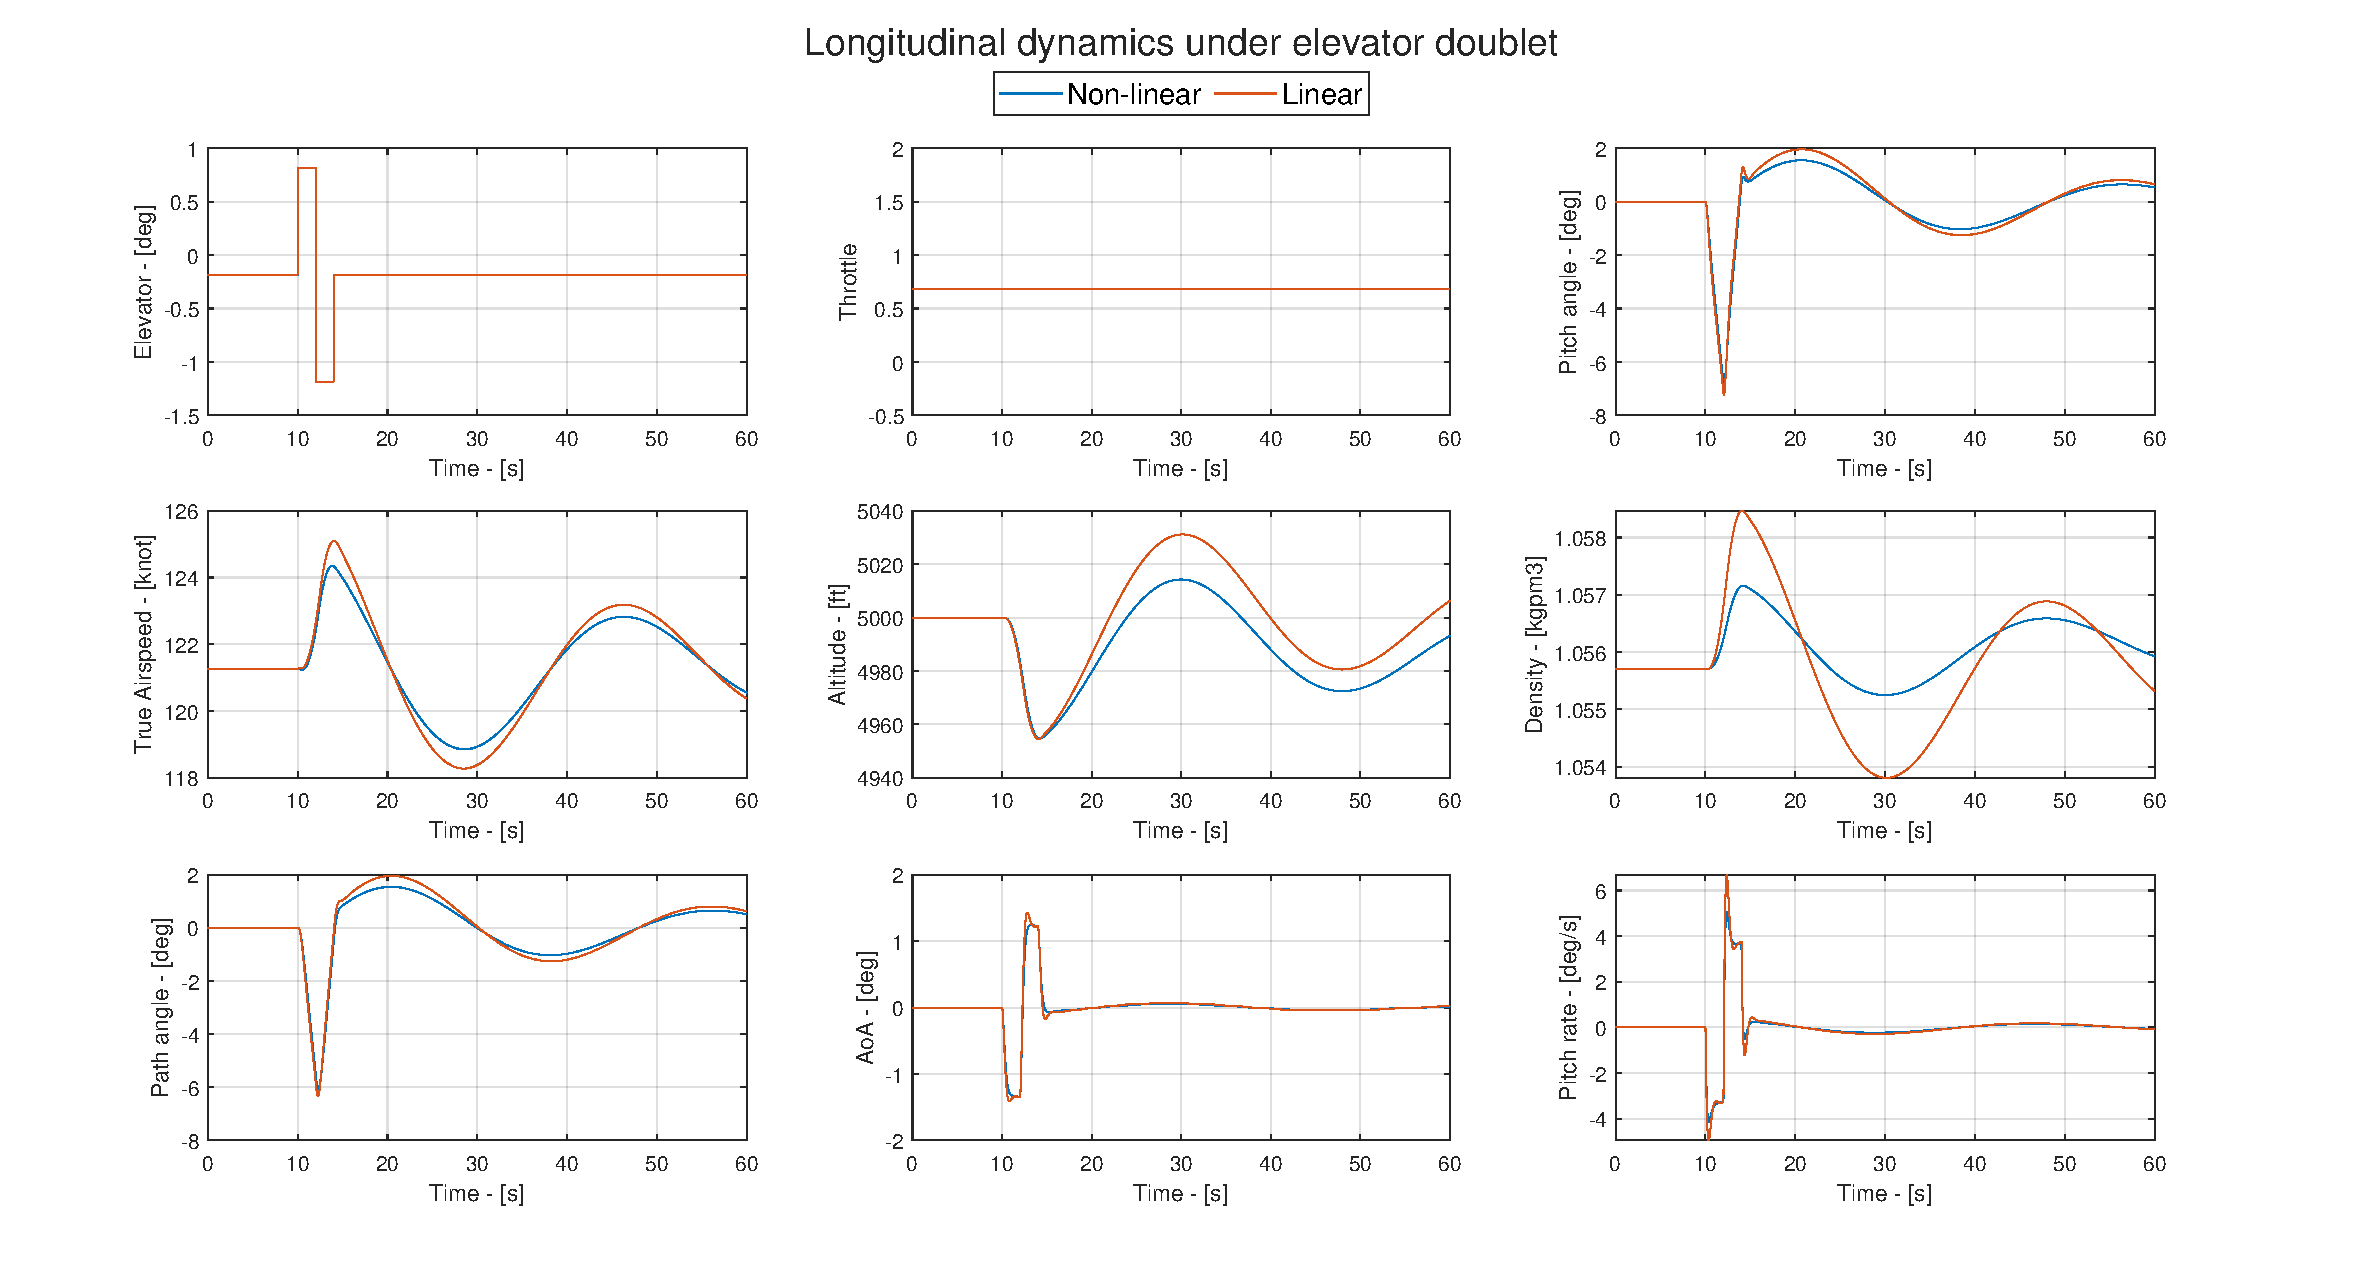
\includegraphics[width=7in]{figs/elevator_doublet.pdf}%
\caption{Longitudinal dynamics under elevator doublet: nonlinear vs linear models.}
\label{fig:elevator_doublet}
\end{figure*}

\subsection{Open-loop and closed-loop response}
The open-loop and closed-loop (with unity feedback) systems are checked against a step response of 0.2 $rad$ ($\approx$ 11.46 $deg$). Figure \ref{fig:ol_step} and \ref{fig:cl_step} show the open-loop and closed-loop step responses, respectively. The open-loop response is marginally stable, but difficult to control and the steady-state error is also large. The unity feedback even makes the system unstable.

\begin{figure}[!t]
\centering
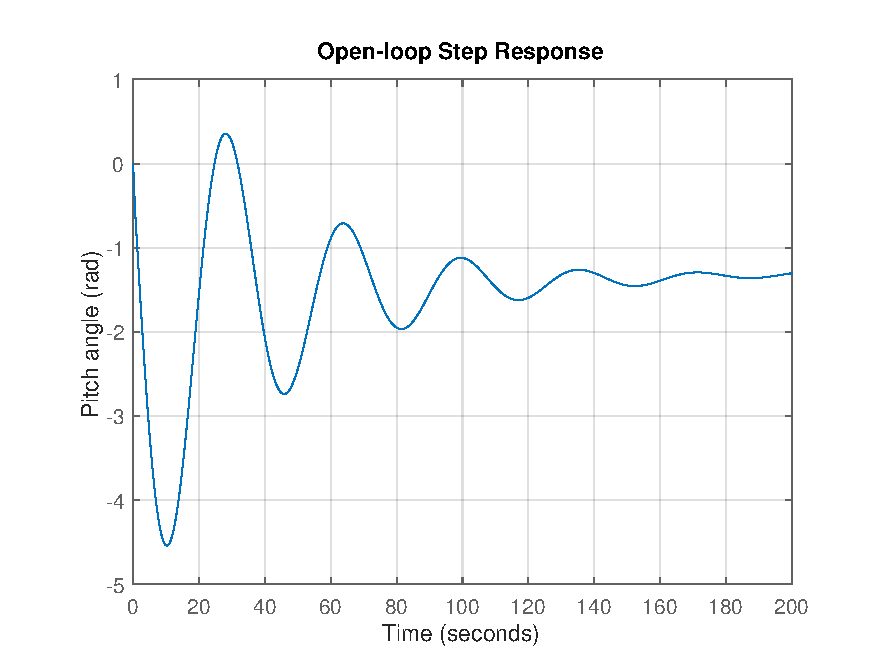
\includegraphics[width=2.5in]{figs/open_loop_step_response.pdf}
\caption{Step response of the open-loop system.}
\label{fig:ol_step}
\end{figure}

\begin{figure}[!t]
\centering
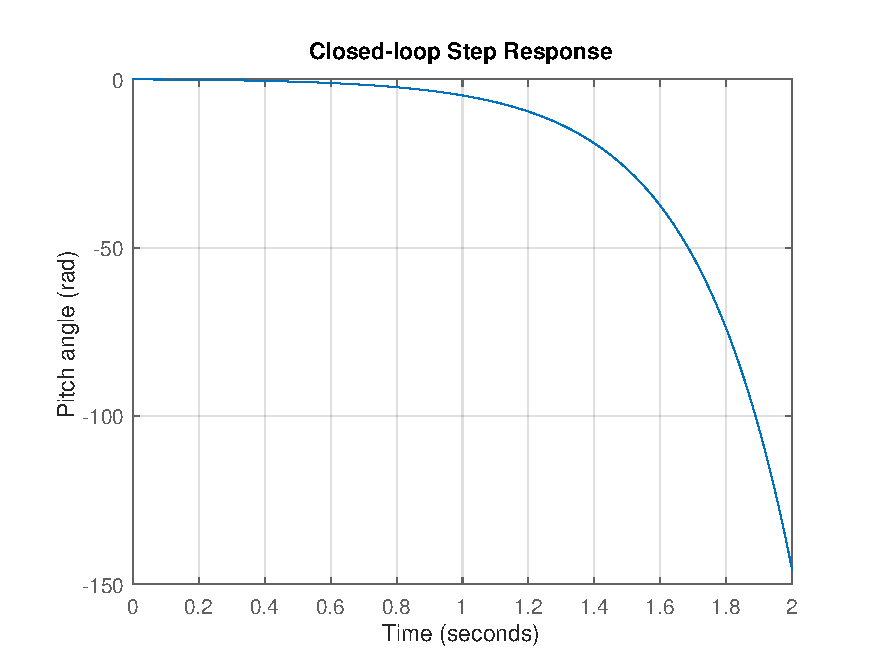
\includegraphics[width=2.5in]{figs/closed_loop_step_response.pdf}
\caption{Step response of the closed-loop with unity feedback.}
\label{fig:cl_step}
\end{figure}

\section{Traditional method}
\subsection{Static PID controller}
Proportional-Integral-Derivative (PID) control is a well-established control method that has been used across engineering fields due to its simplicity. By tuning the proper gain values, the performance of a closed-loop system can be enhanced. The mathematical formulation of the PID in this project is written as:
\begin{equation}
C_{\mathrm{PID}}(s) = K_{\mathrm{P}} + \frac{K_{\mathrm{I}}}{s} + \frac{K_{\mathrm{D}}\,s}{s/N+1}
\end{equation}
where $K_{\mathrm{P}}$ is the proportional gain, $K_{\mathrm{I}}$ is the integral gain, $K_{\mathrm{D}}$ is the derivative gain, and $N$ is the time filter coefficient taken as a constant 100 in this project.

The schematic of the static PID coupled with aircraft longitudinal dynamics is shown in Figure \ref{fig:pid_scheme}. It is noted that although the system has a multiple outputs, the output being tracked is only the pitch angle. Therefore, the system is essentially still a Single-Input-Single-Output (SISO) model. The input from the throttle is assumed to be constant at the trimmed value, i.e. $\Delta \delta_{\mathrm{t}} = 0$ or $\delta_{\mathrm{t}_0} = 0.6792$. It is also noted that the gains $K_{\mathrm{P}}$, $K_{\mathrm{I}}$, and $K_{\mathrm{D}}$ are constant and tuned beforehand.

\begin{figure*}[!t]
\centering
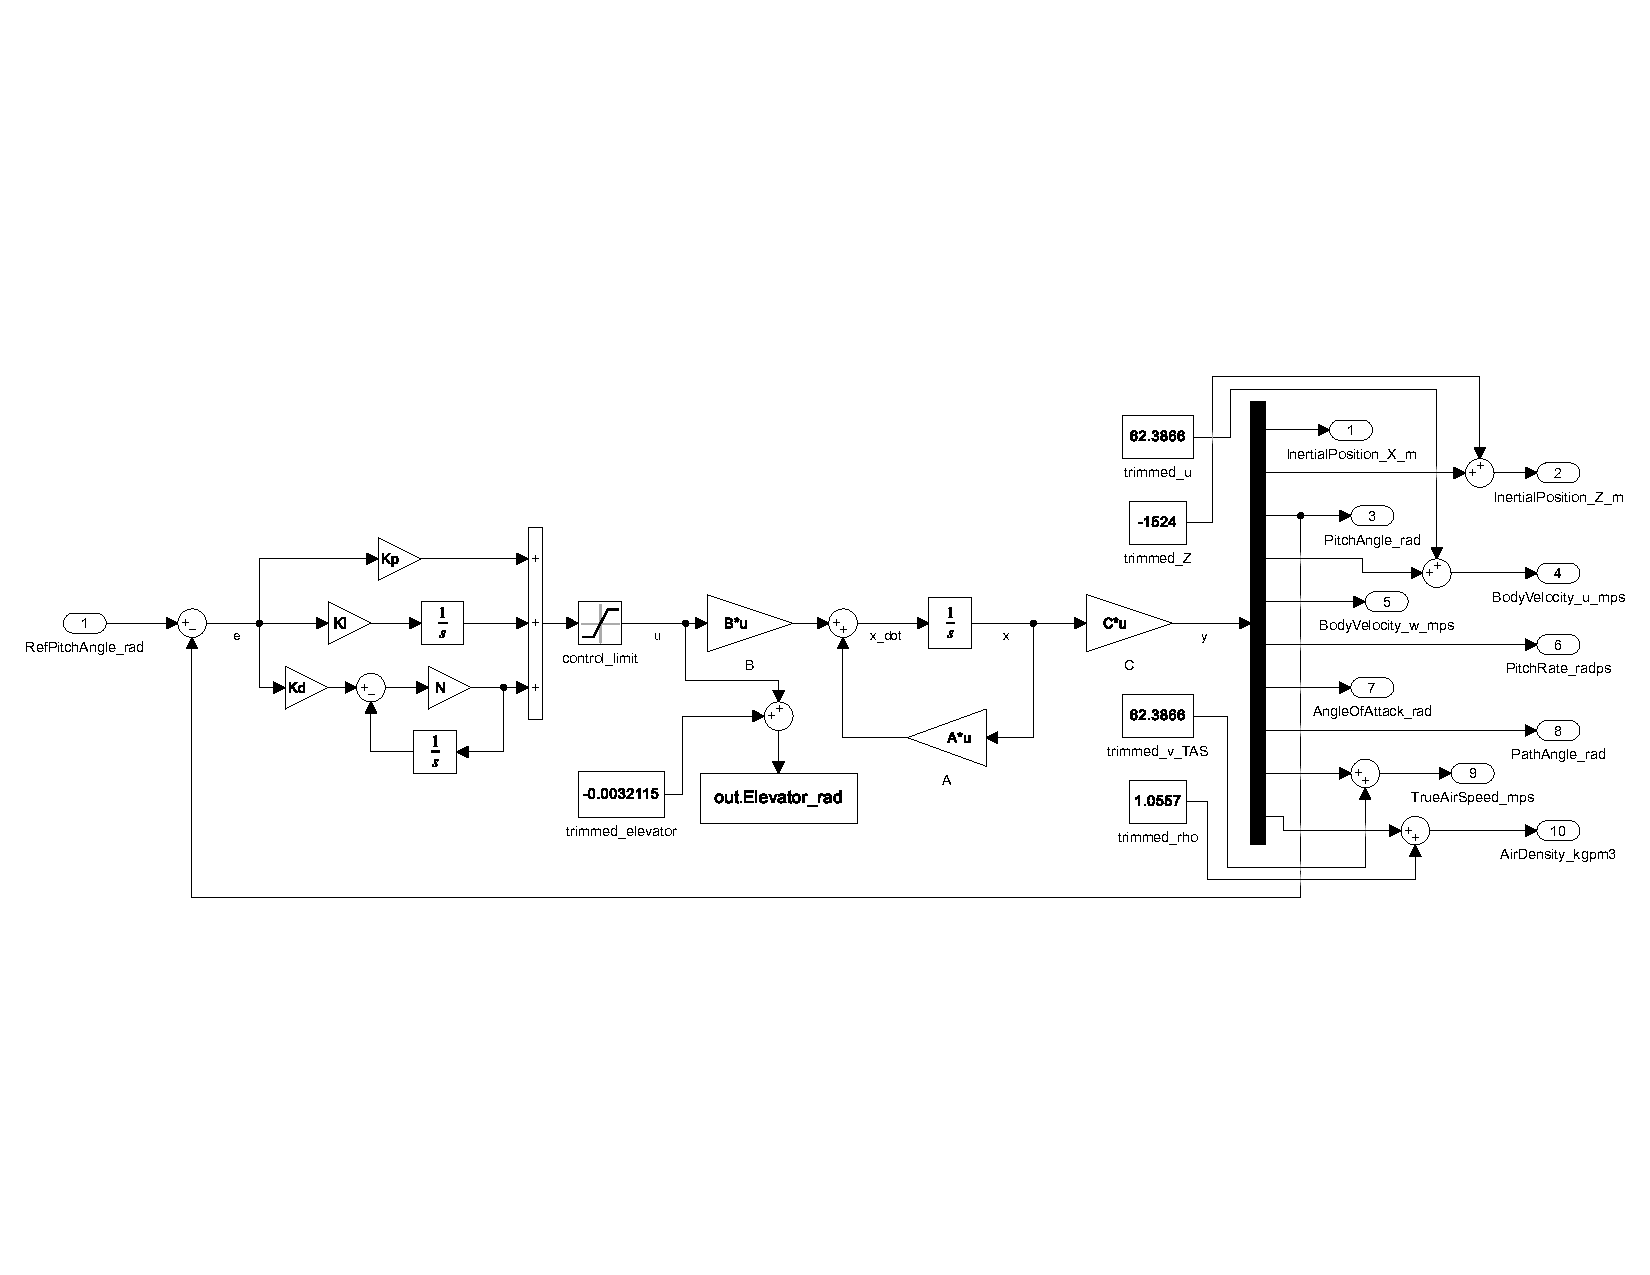
\includegraphics[width=7in]{figs/pid_scheme.pdf}%
\caption{Static PID control coupled with longitudinal dynamic system: tracking the reference pitch angle.}
\label{fig:pid_scheme}
\end{figure*}

\subsection{Time-domain performance}
A controller should be designed to have the following criteria under a $0.2rad$ step input: a) rise time $<2$ seconds, b) settling time $<10$ seconds, c) overshoot $<10\%$, and d) steady-state error $<2\%$. PID controller with the static gains listed in Table \ref{tab:different_pid_performance} are explored. In PID\_1, the derivative gain is zero. The rise and settling times match the criteria, while the overshoot of $22.4851\%$ does not meet the $<10\%$ criterion. Thus, the integral gain is iteratively reduced until it reaches $K_{\mathrm{I}}=-0.3$ in PID\_4, where it satisfies all our criteria. But, when the derivative gain is introduced in PID\_5, the system's overshoot is reduced to $4.3979\%$. It is noted that all the systems have steady-state error $<2\%$.

\begin{table*}[!t]
\caption{Time-domain performance of PID with different static gains}
\label{tab:different_pid_performance}
\centering
\begin{tabular}{|c||c||c||c||c||c||c|c|}
\hline
PID Name & $K_{\mathrm{P}}$  & $K_{\mathrm{I}}$ & $K_{\mathrm{D}}$ & Rise Time (s) & Settling Time (s) & Overshoot (\%) & Steady-State Error (\%) \\
\hline
PID\_1 & $-1.0$ & $-1.0$ & $0.0$ & $0.2370$ & $3.1187$ & $22.4851$ & $0.5179$ \\
\hline
PID\_2 & $-1.0$ & $-0.8$ & $0.0$ & $0.2429$ & $3.5128$ & $19.0088$ & $0.6609$ \\
\hline
PID\_3 & $-1.0$ & $-0.6$ & $0.0$ & $0.2488$ & $4.0294$ & $15.6260$ & $0.8921$ \\
\hline
PID\_4 & $-1.0$ & $-0.3$ & $0.0$ & $0.2648$ & $5.0701$ & $9.9522$ & $1.4383$ \\
\hline
PID\_5 & $-1.0$ & $-0.3$ & $-0.1$ & $0.2848$ & $4.9752$ & $4.3979$ & $1.1606$ \\
\hline
\end{tabular}
\end{table*}

\subsection{Tracking performance and input limitation}

Figure \ref{fig:tracking_performance_pids} shows the performance of PID with different static gains tracking the 0.2 $rad$ step reference input. As discussed previously, all the static PID controllers succesfully track the reference input. However, this plot does not give any information regarding the requested control input by each controller. Therefore, the input-output dynamics are plotted in Figure \ref{fig:io_pids}. It is observed that PID\_5 requests a high control input from the very beginning: a maximum of $-30^\mathrm{o}$ of elevator deflection. It is noted that our closed-loop system has a saturation model to prevent the controller to give a very high control input, i.e., $-30^\mathrm{o} \leq \Delta \delta_{\mathrm{e}} \leq 30^\mathrm{o}$. If the saturation is removed, PID\_{5} will request around $-100^\mathrm{o}$, which is outside the capability of the mechanical system.

\begin{figure}[!t]
\centering
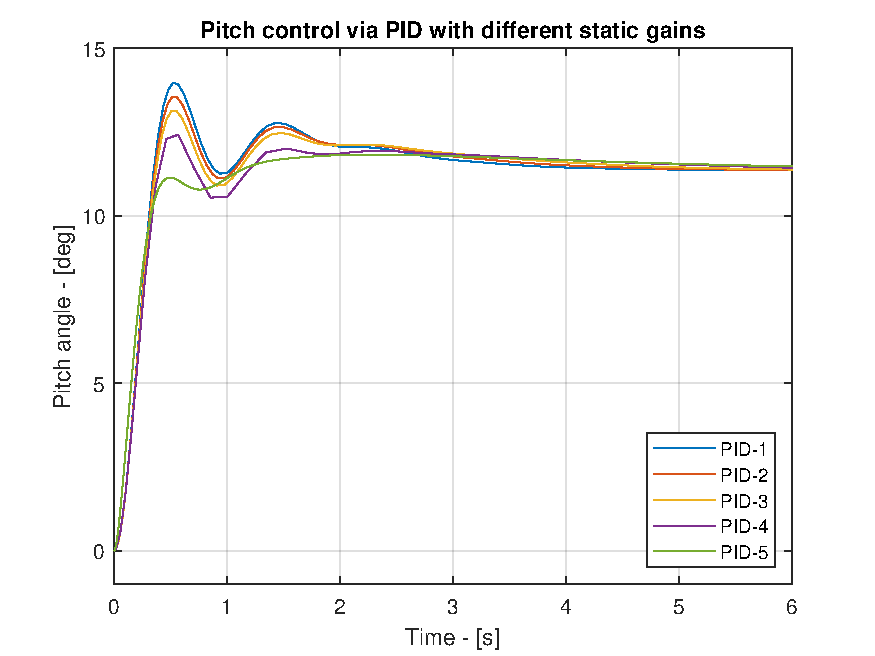
\includegraphics[width=2.5in]{figs/tracking_performance_pids.pdf}
\caption{Tracking performance of PID with different gains.}
\label{fig:tracking_performance_pids}
\end{figure}

\begin{figure*}[!t]
\centering
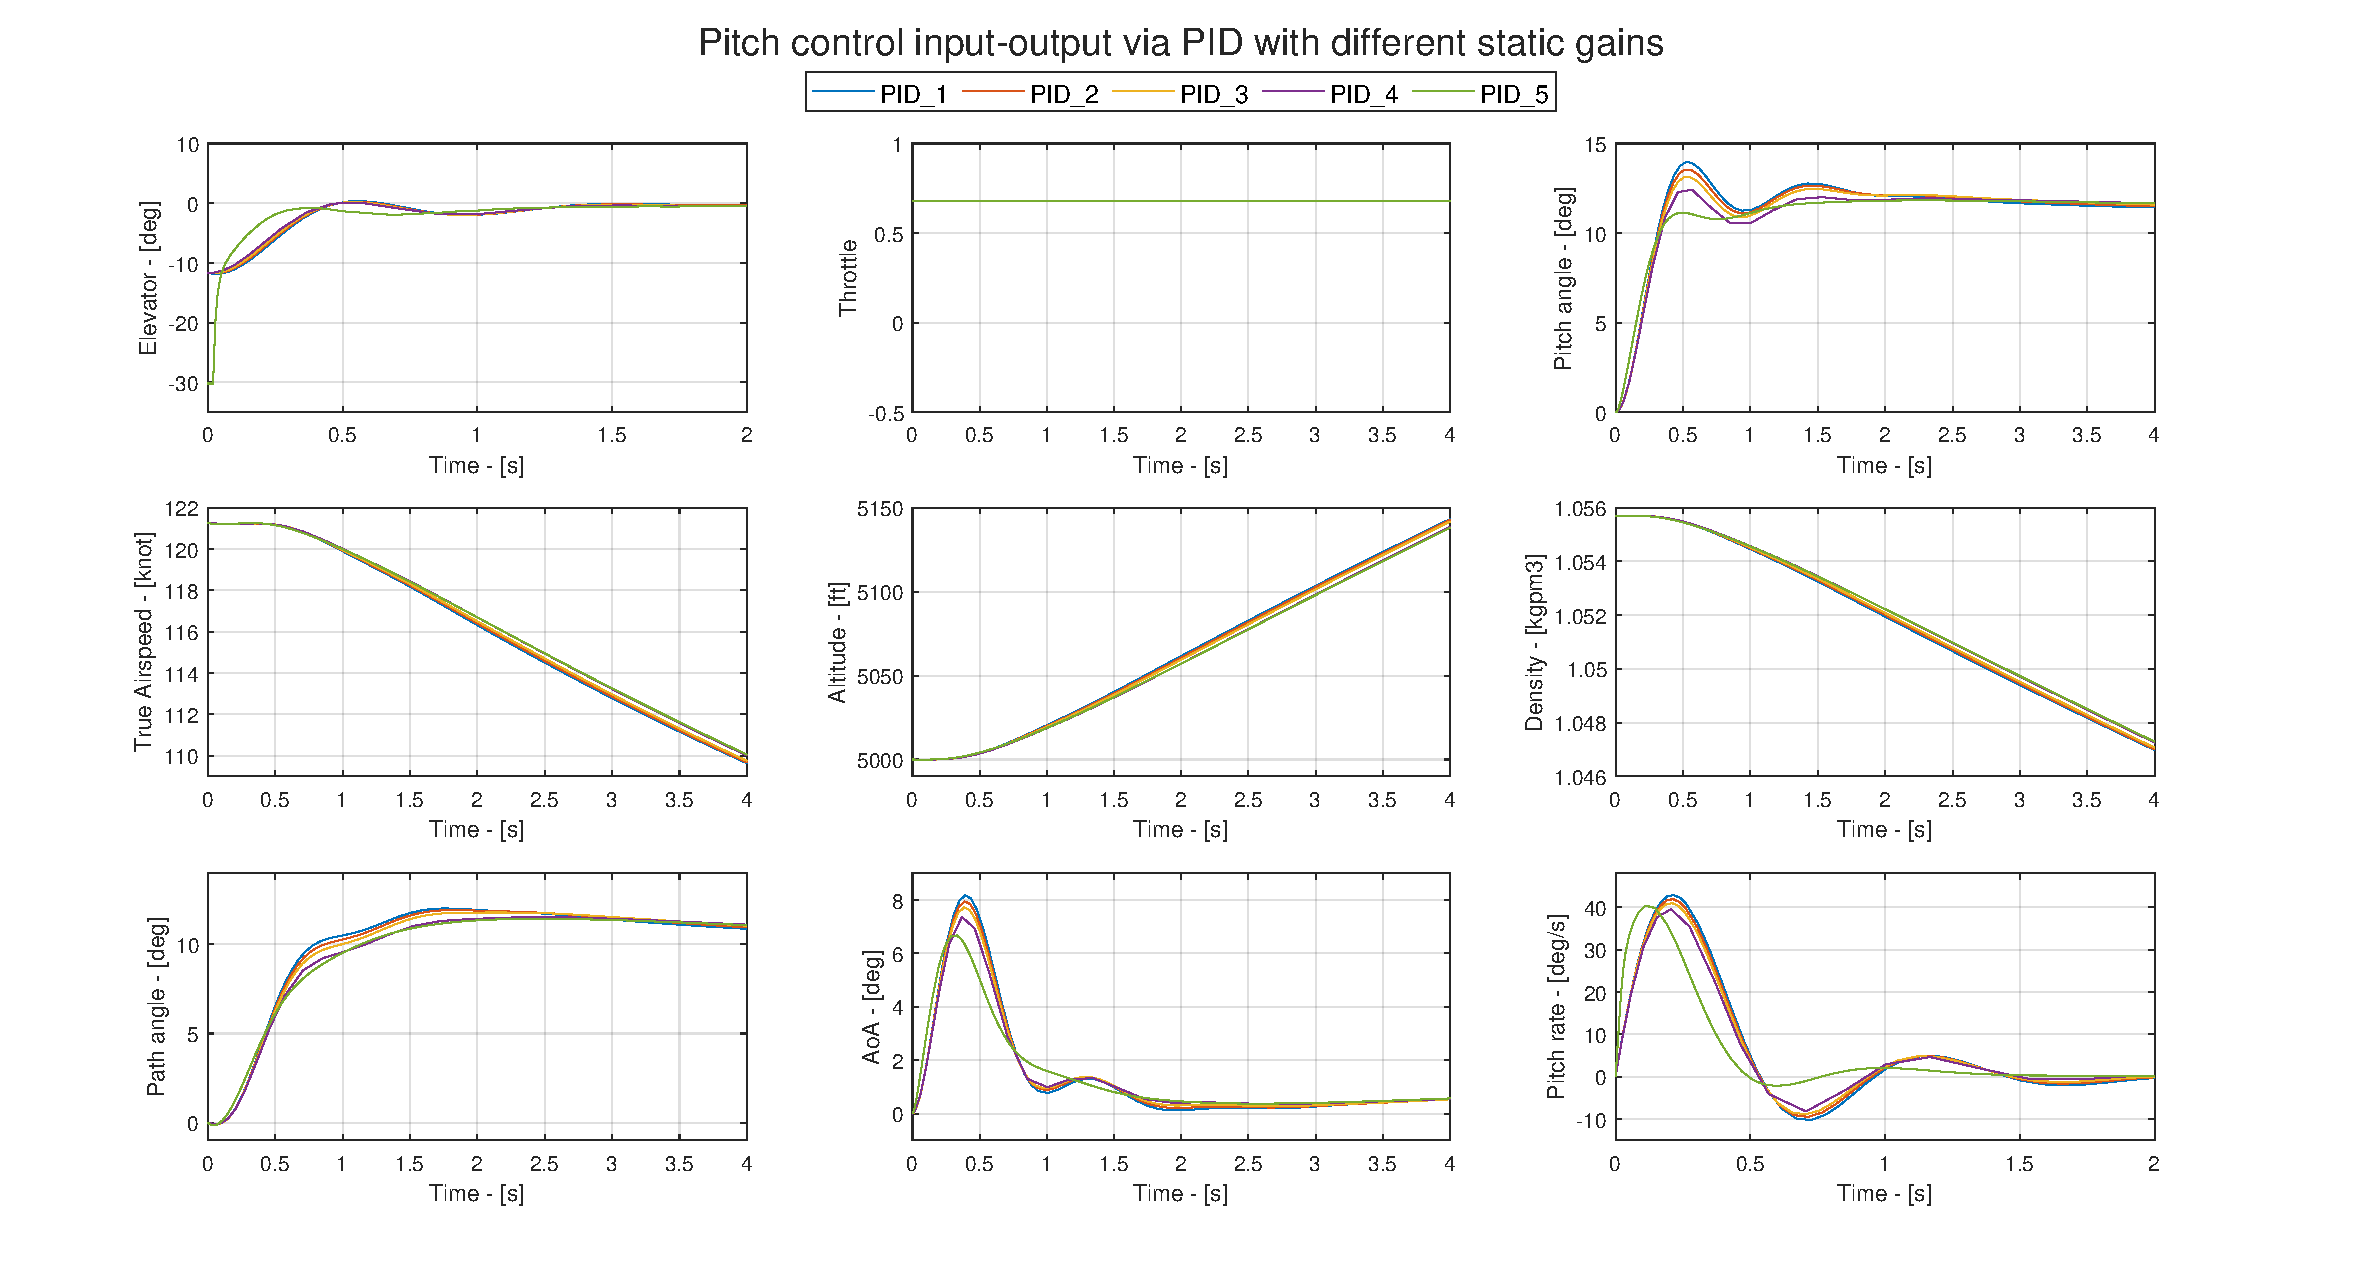
\includegraphics[width=7in]{figs/input_output_pids.pdf}%
\caption{Input-output dynamics of the systems with different static PID gains.}
\label{fig:io_pids}
\end{figure*}

\section{Intelligent method}
\subsection{RL-based adaptive PID controller}
The class of RL algorithm used here is called PPO \cite{ref13}, in which it includes two deep neural networks: action net and value net. Specifically, the action net is trained to map a normalized error of the aircraft pitch (difference between the desired and observed pitch divided by the desired pitch), as an observation, into the three PID gains as its actions. Simultaneously, the value net is trained to map the given observation and actions into a reward value.

\subsection{Training and validation of different neural net architectures}
The key idea of any RL algorithms is to train an agent (action net) by letting it interact with the environment with the purpose of cumulating the highest reward possible. After training, the agent can be deployed to perform the specific task it was trained for. In this project, the agent interacts with the aircraft longitudinal system + PID controller as its environment by giving actions (PID gains) with the purpose of obtaining the highest reward. The environment starts with $\theta_{\mathrm{obs}}=0^\mathrm{o}$, and the desired pitch is $-0.5\leq\theta_{\mathrm{des}}\leq0.5$, measured in $radians$. The reward function is defined as:
\begin{equation}\label{eq:reward_function}
rew = - \left(\frac{\theta_{\mathrm{des}}-\theta_{\mathrm{obs}}}{\theta_{\mathrm{des}}}\right)^2 - \left(\frac{\Delta\delta_{\mathrm{e}}}{\Delta\delta_{\mathrm{e,max}}}\right)^2 - 10.0\delta_{\mathrm{term}} + 1.0
\end{equation}

The first term corresponds to the punishment for deviating from the desired pitch value, the second term dictates the agent to act efficiently, the third term is the punishment if the $|\theta_{\mathrm{obs}}|>=90^{o} (\delta_{term}=1)$, while the last term is the reward for advancing further in timesteps. The maximum time and the discrete timestep are set to $6 s$ and $0.01 s$, respectively.

Unlike traditional supervised learning algorithms, RL (specifically PPO), collects data and trains its networks simultaneously, which is referred to as an on-policy algorithm. During the training, a separate set of environments are used as validation set to evaluate how well the agent performs the task considered (pitch control). The training is stopped when the mean reward collected by the agent in the validation set reach a certain value. In this project, this value is set to $580$, having known that the maximum reward is $600$ per episode. This way, the training will not be too exhaustive, while the trained agent is good enough at performing its task.

\begin{figure}[!t]
\centering
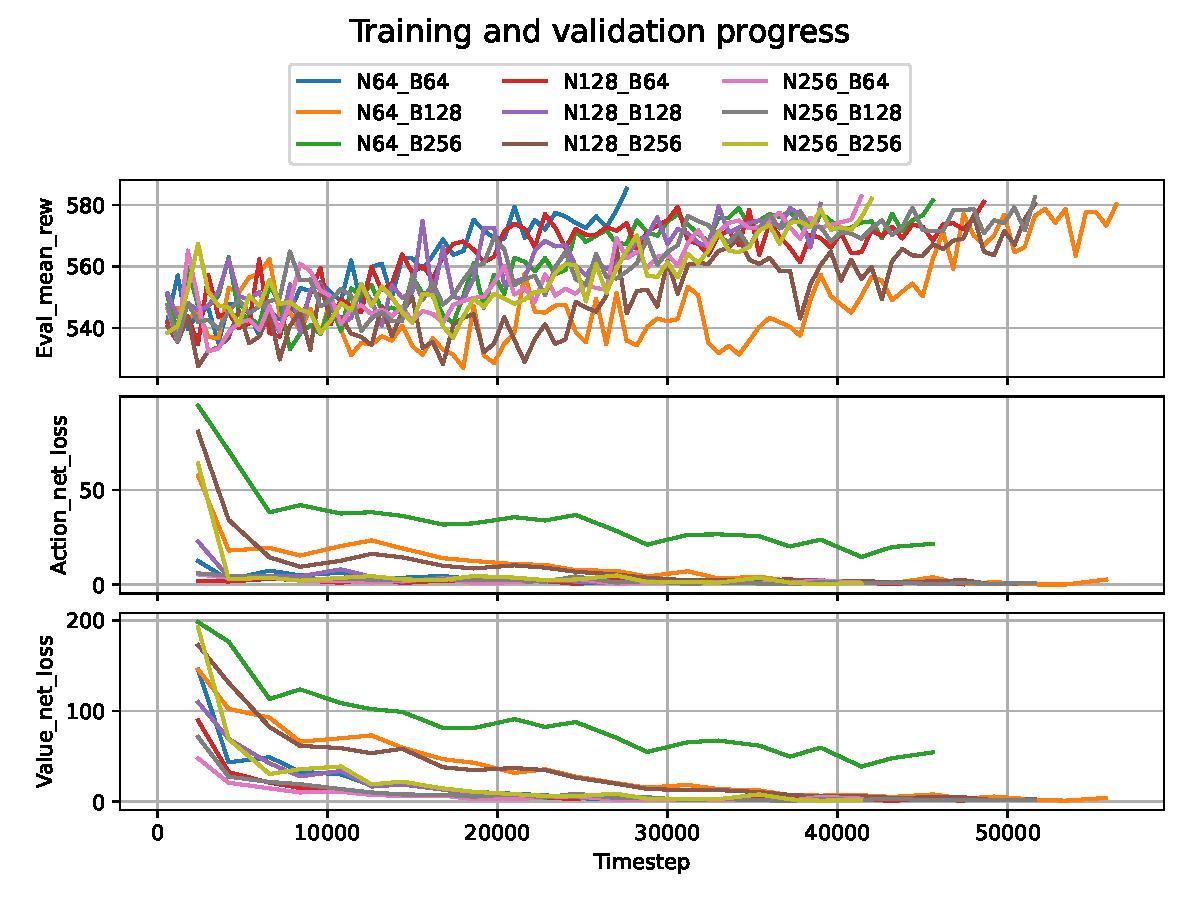
\includegraphics[width=3.2in]{figs/training_and_validation_progress.pdf}
\caption{Training and validation progress.}
\label{fig:training_and_validation_progress}
\end{figure}

Different architectures for both the action and value nets are investigated by adjusting the number of neurons (N) in each hidden layer of the nets to be either $64$, $128$, or $256$. The batchsize (B) is also varied to be either $64$, $128$, or $256$. The number of hidden layers is kept at $2$ with $tanh$ activation function. The action net output is clipped between $[-1,1]$ and rescaled to be between $[-3,0]$ to produce the PID gains.

Figure \ref{fig:training_and_validation_progress} shows how the training progresses for each architecture. It is observed that the training losses for both action and value nets are decreasing, while all the agents succesfully reach the mean reward threshold in the validation sets. The required training timesteps is also summarized in Table \ref{tab:different_rl_performance}. The less the timesteps, the faster the training is, i.e., the fastest to train is the N64\_B64, while the slowest is the N64\_B128.

The training is performed using stable-baselines3 \cite{ref14}. Subsequently, the trained policy (action net) is saved as a pytorch model \cite{ref15}, which can be called in Simulink as a toolbox to predict the adaptive PID gains, shown in Figure \ref{fig:rl_based_adaptive_pid_scheme}. It is noted that the PID gains are changing depending on the observation (normalized pitch error).

\subsection{Time-domain performance: testing}
After a trained policy is obtained and deployed in the Simulink model (see Figure \ref{fig:rl_based_adaptive_pid_scheme}), the testing is performed under a $0.2rad$ step input, as previously done with the static PID. The controllers' step-response characteristics are summarized in Table \ref{tab:different_rl_performance}, with the same criteria as before. It can be observed that all trained policies with different net architectures, except the one with 64 neurons and 128 batchsize (N64\_B128), satisfy all the criteria with the rise time $<0.5s$, the settling time $<6s$, the overshoot $<10\%$, and the steady-state error $<1\%$. The N64\_B128 policy fails to satisfy the $<10\%$ overshoot criterion by a small amount of violation.

\begin{figure*}[!t]
\centering
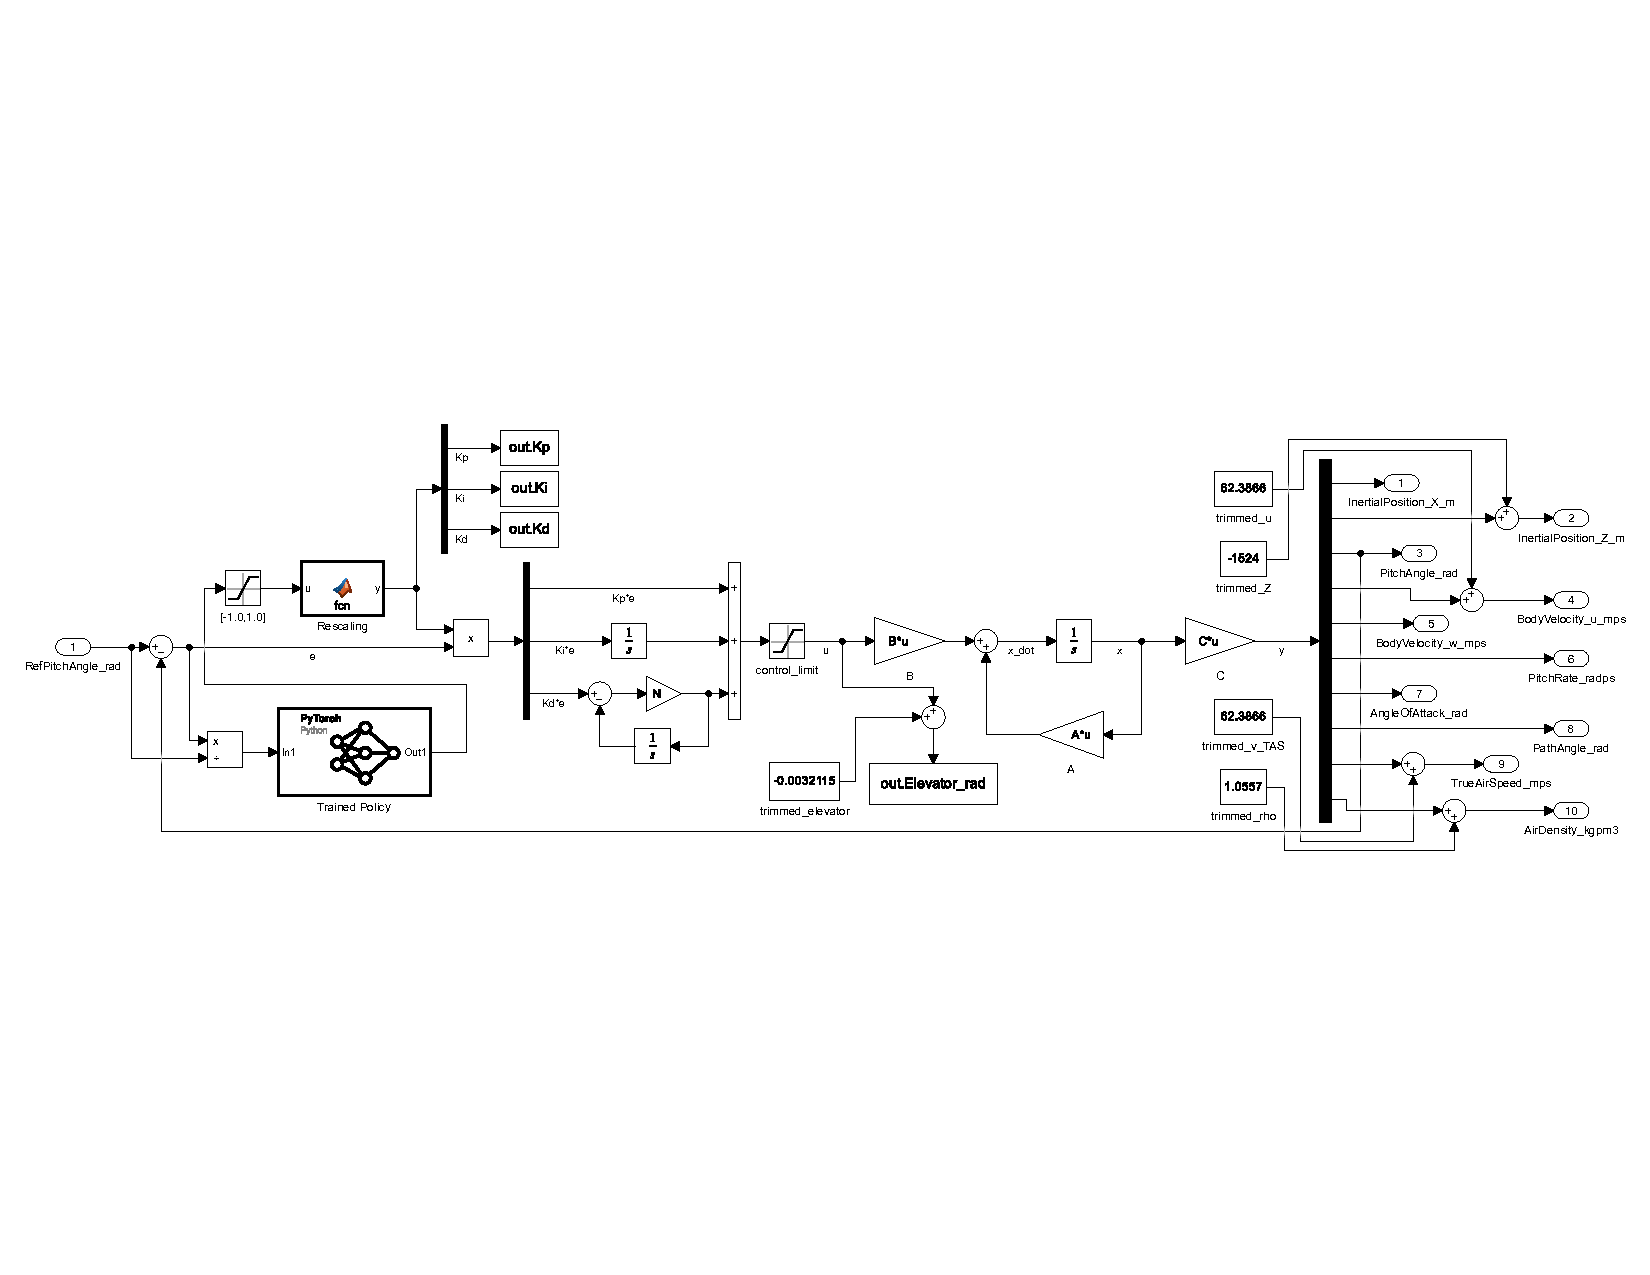
\includegraphics[width=7in]{figs/rl_based_adaptive_pid_scheme.pdf}%
\caption{RL-based adaptive PID controller being deployed for tracking the aircraft pitch angle.}
\label{fig:rl_based_adaptive_pid_scheme}
\end{figure*}

\begin{table*}[!t]
\caption{Time-domain performance of RL-based adaptive PID with different neural network architectures}
\label{tab:different_rl_performance}
\centering
\begin{tabular}{|c||c||c||c||c||c||c|c|}
\hline
No & N\_neurons & Batchsize & Req. Training Timesteps & Rise Time (s) & Settling Time (s) & Overshoot (\%) & Steady-State Error (\%) \\
\hline
$1$ & $64$ & $64$ & $27600$ & $0.1220$ & $3.7462$ & $4.2309$ & $0.4396$ \\
\hline
$2$ & $64$ & $128$ & $56400$ & $0.1543$ & $5.1725$ & $10.6501$ & $0.9282$ \\
\hline
$3$ & $64$ & $256$ & $45600$ & $0.1606$ & $3.3941$ & $8.3370$ & $0.3259$ \\
\hline
$4$ & $128$ & $64$ & $48600$ & $0.4991$ & $4.7149$ & $9.7276$ & $0.5768$ \\
\hline
$5$ & $128$ & $128$ & $39000$ & $0.1371$ & $3.9755$ & $4.9228$ & $0.4647$ \\
\hline
$6$ & $128$ & $256$ & $51600$ & $0.4823$ & $3.9777$ & $4.5844$ & $0.4058$ \\
\hline
$7$ & $256$ & $64$ & $41400$ & $0.1269$ & $3.8706$ & $7.6882$ & $0.2827$ \\
\hline
$8$ & $256$ & $128$ & $51600$ & $0.1313$ & $4.4782$ & $9.4892$ & $0.6104$ \\
\hline
$9$ & $256$ & $256$ & $42000$ & $0.1280$ & $5.8598$ & $7.0842$ & $0.6672$ \\
\hline
\end{tabular}
\end{table*}

\subsection{Tracking performance and adaptive PID gains trajectories}
Based on the previous results, three trained policies are selected for comparison. The pitch trajectories by these selected trained policies are depicted in Figure \ref{fig:tracking_performance_rl_adaptive_pids}, while Figure \ref{fig:io_rl_pids} illustrates a more comprehensive input-output dynamics. It is observed that the trained policies request a maximum control input $|\Delta\delta_{\mathrm{e}}|=30^\mathrm{o}$ at $t<0.5s$, resulting in short rise times. In Figure \ref{fig:adaptive_pid_gains}, the trajectories of PID gains over time are demonstrated. Each set of PID gains displays a transient behavior $t<0.5s$ before converging to a near-steady state towards the end. These varying PID gains contribute to the great time-domain performances.

\begin{figure}[!t]
\centering
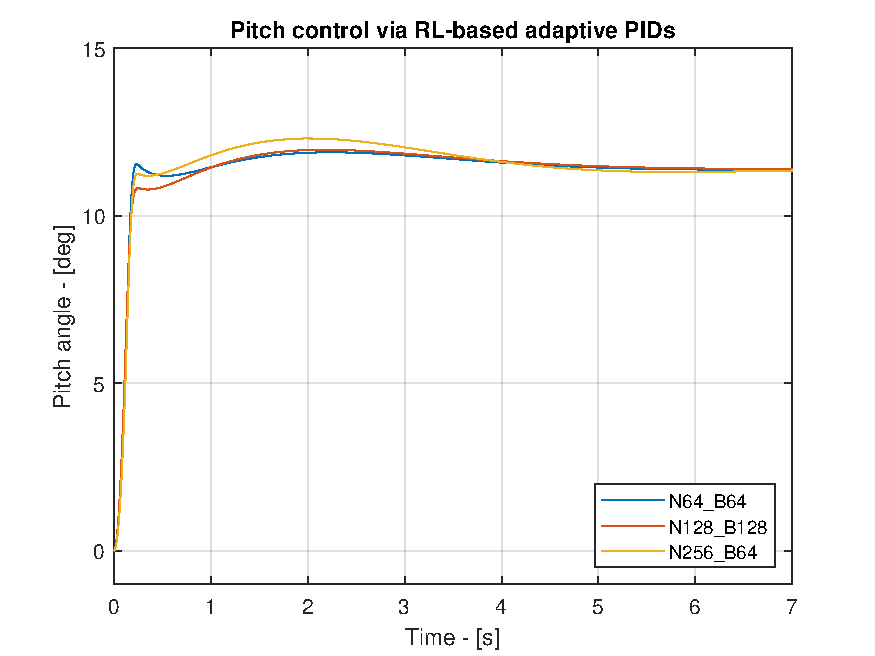
\includegraphics[width=2.6in]{figs/tracking_performance_rl_adaptive_pids.pdf}
\caption{Tracking performance of selected RL-based PIDs.}
\label{fig:tracking_performance_rl_adaptive_pids}
\end{figure}

\begin{figure*}[!t]
\centering
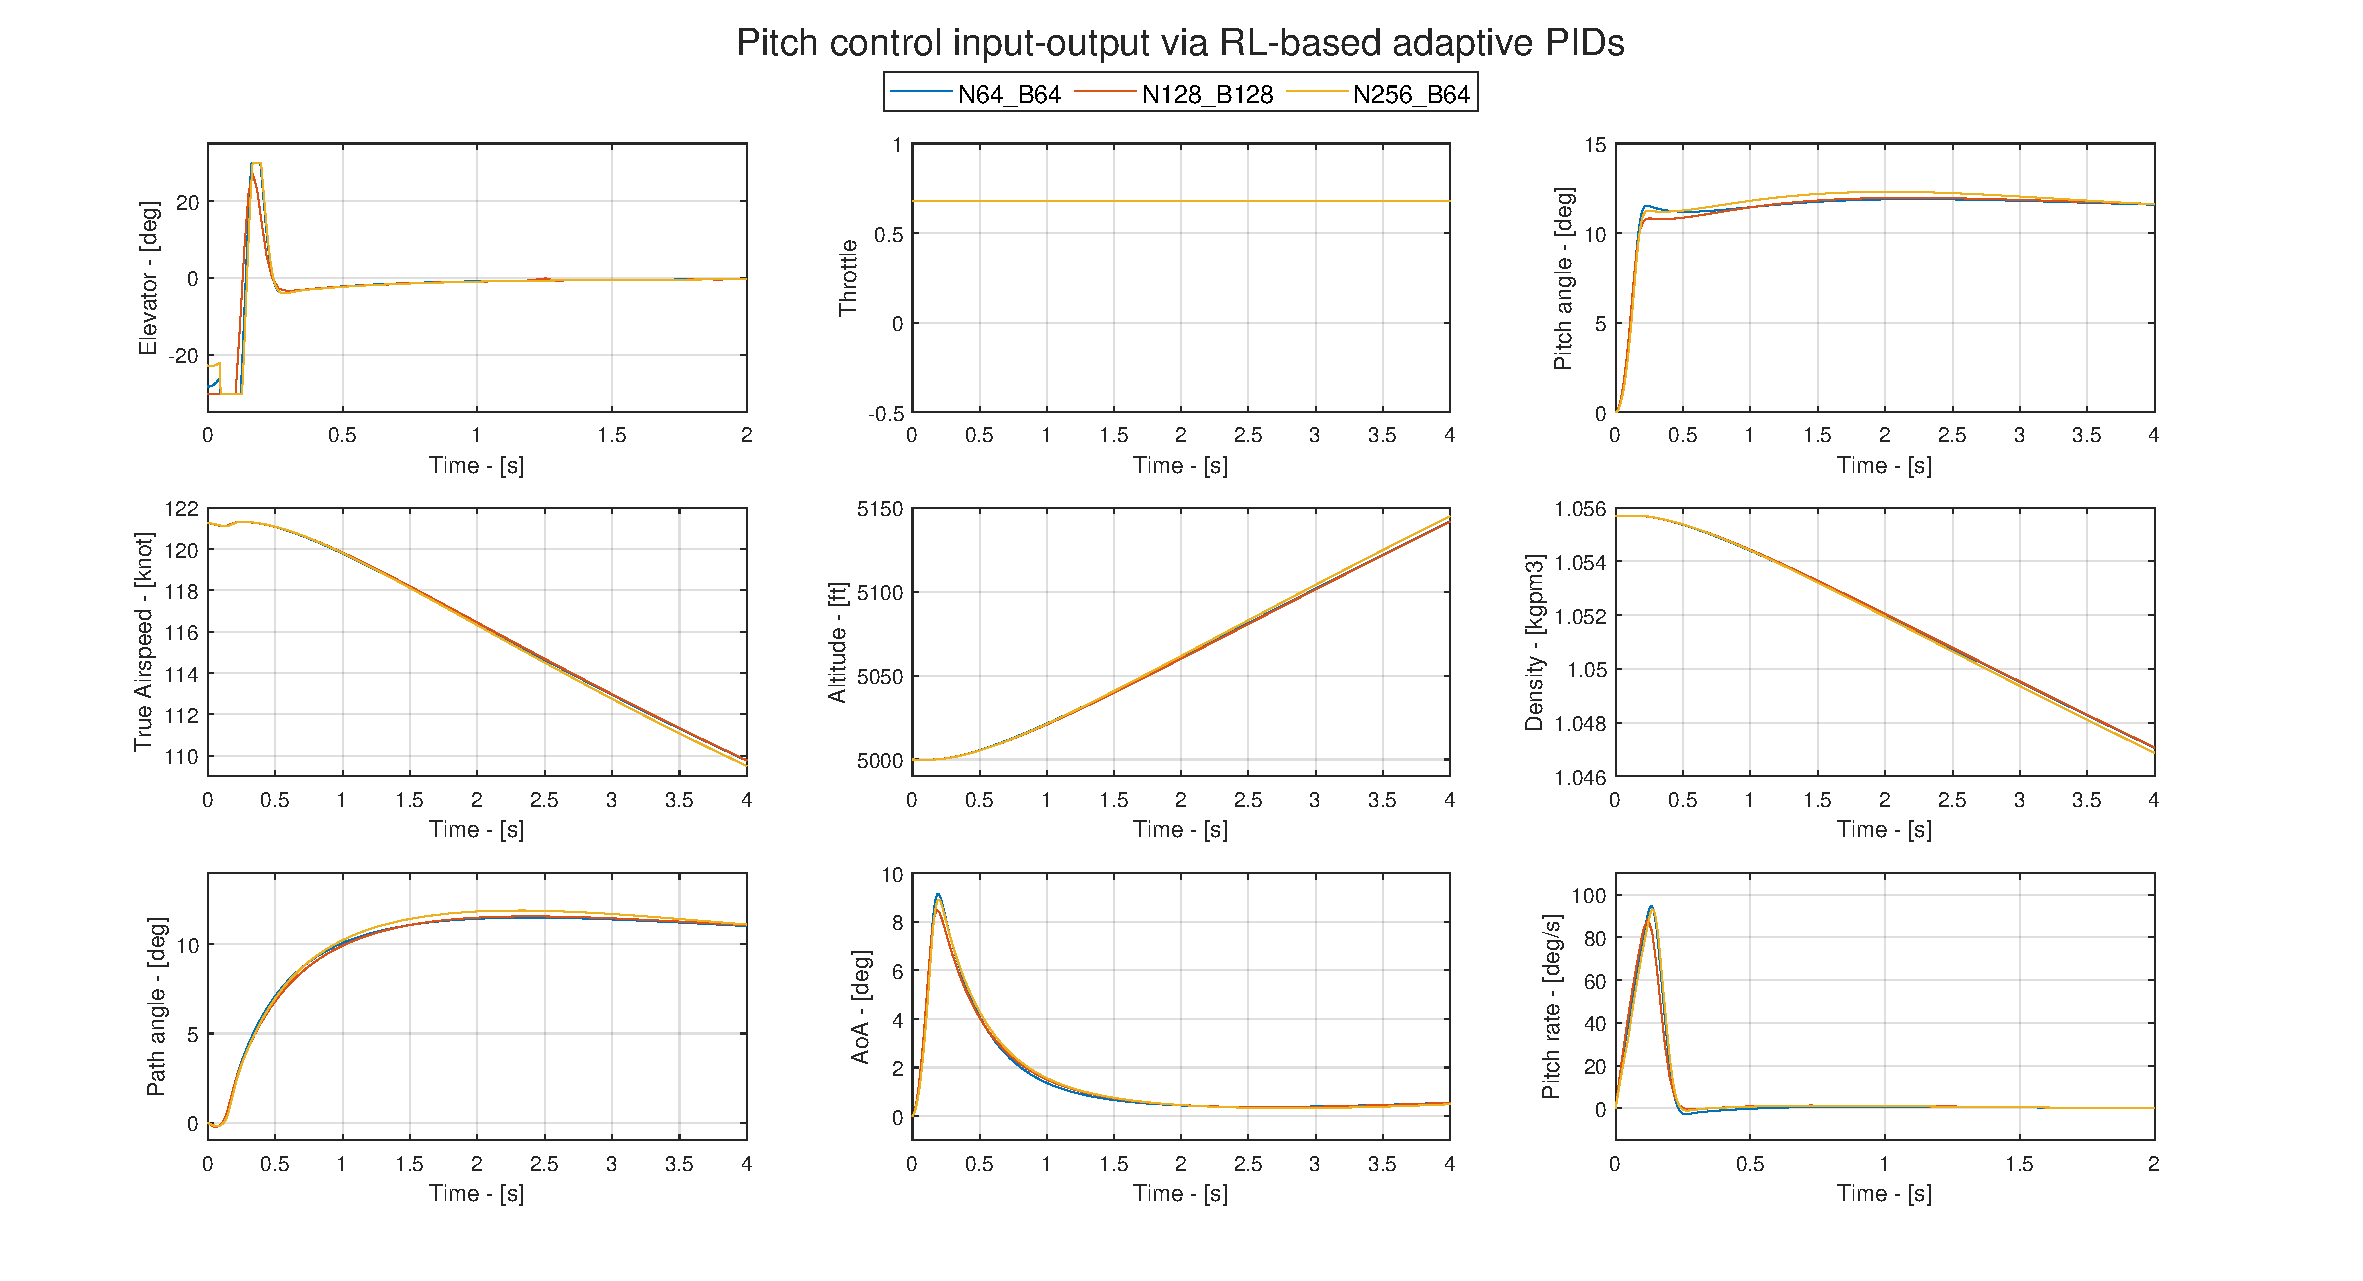
\includegraphics[width=7in]{figs/input_output_rl_pids.pdf}%
\caption{Input-output dynamics of the systems with RL-based adaptive PIDs.}
\label{fig:io_rl_pids}
\end{figure*}

\begin{figure}[!t]
\centering
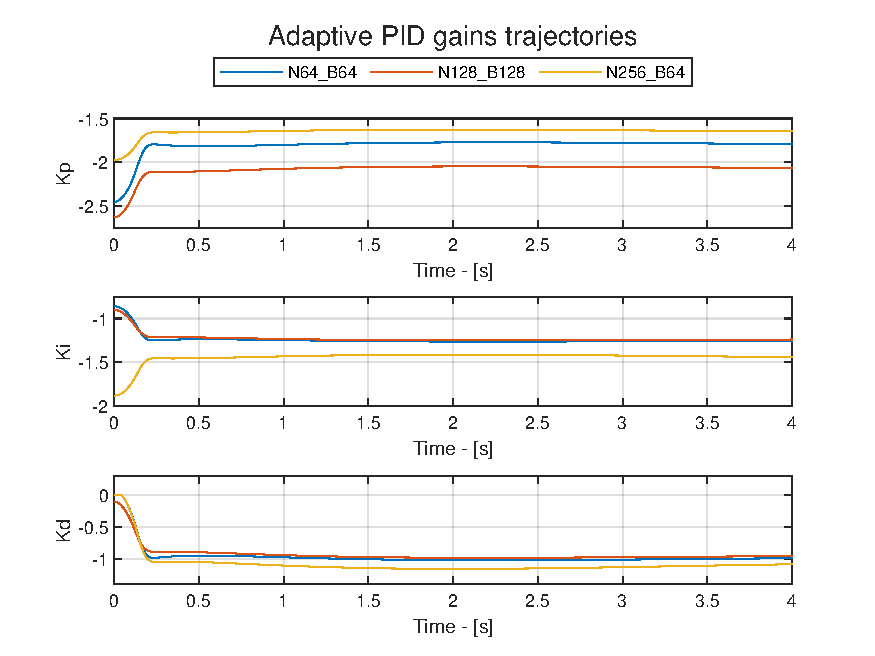
\includegraphics[width=3.5in]{figs/adaptive_pid_gains.pdf}
\caption{Adaptive PID gains for selected trained policies.}
\label{fig:adaptive_pid_gains}
\end{figure}

\section{Conclusion and future work}
In this project, a 6-DOF non-linear aircraft dynamics model based on Cessna-172 stability derivatives is developed from first principles. Subsequently, a linearized system is derived and used to design PID controllers for tracking a desired pitch angle. Two methods are used: traditional and intelligent. In the traditional method, manual tuning of static PID gains is conducted, while the intelligent method uses an RL algorithm to predict adaptive PID gains. The former relies on a trial-and-error process assuming familiarity with the dynamic model, whereas the latter involves crafting an appropriate reward function and network architectures without requiring knowledge about the dynamic model (model-free, data-driven). Future work should investigate the effectiveness of adaptive PID gains in scenarios involving time-varying uncertainties, e.g. wind gusts. Additionally, it should assess off-design situations where static gains could potentially exhibit degradred performance.

\newpage

\begin{thebibliography}{1}
\bibliographystyle{IEEEtran}

\bibitem{ref1}
R.C. Nelson, ``Flight Stability and Automatic Control,'' McGraw Hill, Second Edition, 1998.

\bibitem{ref2}
Bernard Etkin, and Lloyd Duff Reid, ``Dynamics of Flight, Stability and Control,'' McGrawHill, Third Edition, 1996.

\bibitem{ref3}
Duan, M., Cesnik, C. E. S., Kolmanovsky, I. V., and Vetrano, F., ``Control-Oriented Modeling for Flexible Aircraft,'' \textit{Journal of Aircraft}, Vol. 61, No. 1, 2024, pp. 183–195. https://doi.org/10.2514/1.C037049

\bibitem{ref4}
S. N. Deepa and G. Sudha, ``Longitudinal control of aircraft dynamics based on optimization of PID parameters,'' \textit{Thermophys. Aeromech.}, vol. 23, no. 2, pp. 185–194, 2016, doi: 10.1134/S0869864316020049.

\bibitem{ref5}
Vishal and J. Ohri, ``GA tuned LQR and PID controller for aircraft pitch control,'' presented at \textit{the 2014 IEEE 6th India International Conference on Power Electronics (IICPE)}, Kurukshetra, India: IEEE, 2014, pp. 1–6. doi: 10.1109/IICPE.2014.7115839.

\bibitem{ref6}
H. Arrosida and M. E. Echsony, ``Aircraft Pitch Control Design using Observer-State Feedback Control,'' \textit{KINETIK}, pp. 263–272, Sep. 2017, doi: 10.22219/kinetik.v2i4.267.

\bibitem{ref7}
A. Mohanty, and E. Schneider, ``Tuning of an Aircraft Pitch PID Controller with Reinforcement Learning and Deep Neural Net,'' (2019). Accessed: Dec. 12, 2024. [Online]. Available: https://cs229.stanford.edu/proj2019aut/data/assignment\_308832\_raw/
26643693.pdf

\bibitem{ref8}
N. Wahid and N. Hassan, ``Self-Tuning Fuzzy PID Controller Design for Aircraft Pitch Control,'' presented at \textit{the 2012 3rd International Conference on Intelligent Systems, Modelling and Simulation (ISMS)}, Kota Kinabalu, Malaysia: IEEE, 2012, pp. 19–24. doi: 10.1109/ISMS.2012.27.

\bibitem{ref9}
Y. Liang, G. Li, M. Xu, J. Zhao, F. Hao, and H. Shi, ``An intelligent control method based on artificial neural network for numerical flight simulation of the basic finner projectile with pitching maneuver,'' \textit{Defence Technology}, vol. 32, pp. 663–674, 2024, doi: 10.1016/j.dt.2023.07.012.

\bibitem{ref10}
D. J. Richter, R. A. Calix, and K. Kim, ``A Review of Reinforcement Learning for Fixed-Wing Aircraft Control Tasks,'' \textit{IEEE Access}, vol. 12, pp. 103026–103048, 2024, doi: 10.1109/ACCESS.2024.3433540.

\bibitem{ref11}
T. P. Lillicrap et al., ``Continuous control with deep reinforcement learning,'' 2015, arXiv. doi: 10.48550/ARXIV.1509.02971.

\bibitem{ref12}
C. Kasnakoğlu, ``Investigation of Multi-Input Multi-Output Robust Control Methods to Handle Parametric Uncertainties in Autopilot Design,'' \textit{PLoS ONE}, vol. 11, no. 10, p. e0165017, Oct. 2016, doi: 10.1371/journal.pone.0165017.

\bibitem{ref13}
J. Schulman, F. Wolski, P. Dhariwal, A. Radford, and O. Klimov, “Proximal Policy Optimization Algorithms,” 2017, arXiv. doi: 10.48550/ARXIV.1707.06347.

\bibitem{ref14}
A. Raffin, A. Hill, A. Gleave, A. Kanervisto, M. Ernestus, and N. Dormann, ``Stable-Baselines3: Reliable Reinforcement Learning Implementations,'' Journal of Machine Learning Research, vol. 22, no. 268, pp. 1–8, 2021, Accessed: Dec. 12, 2024. [Online]. Available: http://jmlr.org/papers/v22/20-1364.html

\bibitem{ref15}
A. Paszke et al., ``PyTorch: An Imperative Style, High-Performance Deep Learning Library,'' 2019, arXiv. doi: 10.48550/ARXIV.1912.01703.

\bibitem{ref16}
``U.S. Standard Atmosphere,'' U.S. Government Printing Office, Washington, D.C., 1976.

\end{thebibliography}

\newpage

{\appendices

\section{Cessna-172 Data \cite{ref12}}\label{apdx:Cessna172-data}

\centering

\vfill\null
\textbf{Wing Data}
\begin{equation}
\mathrm{wing\ area} \quad S = 16.1651\ m
\end{equation}
\begin{equation}
\mathrm{wing span} \quad b = 10.9118\ m
\end{equation}
\begin{equation}
\mathrm{MAC} \quad c = 1.4935\ m
\end{equation}

\vfill\null
\textbf{Mass Properties Data}
\begin{equation}
\mathrm{Mass} \quad m = 1043.3\ kg
\end{equation}
\begin{equation}
\mathrm{CG}_{\mathrm{mac}} = 0.3
\end{equation}
\begin{equation}
I_{\mathrm{XX}} = 1285.3\ kgm^2
\end{equation}
\begin{equation}
I_{\mathrm{YY}} = 1824.9\ kgm^2
\end{equation}
\begin{equation}
I_{\mathrm{ZZ}} = 2666.9\ kgm^2
\end{equation}
\begin{equation}
I_{\mathrm{XZ}} = 0.0\ kgm^2
\end{equation}
\begin{equation}
y_{\mathrm{CG}} = 0.0\ m
\end{equation}
\begin{equation}
z_{\mathrm{CG}} = 0.2\ m
\end{equation}
\begin{equation}
g = 9.80665\ m/s^2
\end{equation}

\vfill\null
\textbf{Engine Data}
\begin{equation}
v_{\mathrm{ref}} = 51.4\ m/s
\end{equation}
\begin{equation}
\rho_{\mathrm{ref}} = 1.225\ kg/m^3
\end{equation}
\begin{equation}
n_{\mathrm{v}} = -1.0
\end{equation}
\begin{equation}
n_{\mathrm{\rho}} = 0.75
\end{equation}
\begin{equation}
\alpha_{\mathrm{F}} = 1.0^\mathrm{o}
\end{equation}
\begin{equation}
X_{\mathrm{F}} = 1.0\ m
\end{equation}
\begin{equation}
Z_{\mathrm{F}} = 0.0\ m
\end{equation}
\begin{equation}
T_{\mathrm{max}} = 2070.0\ N
\end{equation}

% \columnbreak
\vfill\null
\textbf{Aerodynamic Derivative: Lift Coefficient}
\begin{equation}
C_{\mathrm{L}_{\mathrm{0}}} = 0.31
\end{equation}
\begin{equation}
C_{\mathrm{L}_{\mathrm{\alpha}}} = 5.143\ /rad
\end{equation}
\begin{equation}
C_{\mathrm{L}_{\mathrm{\delta_{\mathrm{e}}}}} = 0.43\ /rad
\end{equation}
\begin{equation}
C_{\mathrm{L}_{\mathrm{\dot{\alpha}}}} = 0.0\ s/rad
\end{equation}
\begin{equation}
C_{\mathrm{L}_{\mathrm{q}}} = 3.9\ s/rad
\end{equation}

\vfill\null
\textbf{Aerodynamic Derivative: Drag Coefficient}
\begin{equation}
C_{\mathrm{D}_{\mathrm{0}}} = 0.031
\end{equation}
\begin{equation}
C_{\mathrm{D}_{\mathrm{\alpha}}} = 0.13\ /rad
\end{equation}
\begin{equation}
C_{\mathrm{D}_{\mathrm{\delta_{\mathrm{e}}}}} = 0.06\ /rad
\end{equation}

\vfill\null
\textbf{Aerodynamic Derivative: Pitching Moment Coefficient}
\begin{equation}
C_{\mathrm{m}_{\mathrm{0}}} = -0.015
\end{equation}
\begin{equation}
C_{\mathrm{m}_{\mathrm{\alpha}}} = -0.89\ /rad
\end{equation}
\begin{equation}
C_{\mathrm{m}_{\mathrm{\delta_{\mathrm{e}}}}} = -1.28\ /rad
\end{equation}
\begin{equation}
C_{\mathrm{m}_{\mathrm{\dot{\alpha}}}} = -7.27\ s/rad
\end{equation}
\begin{equation}
C_{\mathrm{m}_{\mathrm{q}}} = -12.4\ s/rad
\end{equation}

\vfill\null
\textbf{Aerodynamic Derivative: Side Force Coefficient}
\begin{equation}
C_{\mathrm{Y}_{\mathrm{\beta}}} = -0.31\ /rad
\end{equation}
\begin{equation}
C_{\mathrm{Y}_{\mathrm{\delta_{\mathrm{a}}}}} = 0.0\ /rad
\end{equation}
\begin{equation}
C_{\mathrm{Y}_{\mathrm{\delta_{\mathrm{r}}}}} = 0.187\ /rad
\end{equation}
\begin{equation}
C_{\mathrm{Y}_{\mathrm{p}}} = -0.037\ s/rad
\end{equation}
\begin{equation}
C_{\mathrm{Y}_{\mathrm{r}}} = 0.21\ s/rad
\end{equation}

\vfill\null
\textbf{Aerodynamic Derivative: Rolling Moment Coefficient}
\begin{equation}
C_{\mathrm{l}_{\mathrm{\beta}}} = -0.089\ /rad
\end{equation}
\begin{equation}
C_{\mathrm{l}_{\mathrm{\delta_{\mathrm{a}}}}} = -0.178\ /rad
\end{equation}
\begin{equation}
C_{\mathrm{l}_{\mathrm{\delta_{\mathrm{r}}}}} = 0.0147\ /rad
\end{equation}
\begin{equation}
C_{\mathrm{l}_{\mathrm{p}}} = -0.47\ s/rad
\end{equation}
\begin{equation}
C_{\mathrm{l}_{\mathrm{r}}} = 0.096\ s/rad
\end{equation}

\vfill\null
\textbf{Aerodynamic Derivative: Yawing Moment Coefficient}
\begin{equation}
C_{\mathrm{n}_{\mathrm{\beta}}} = 0.065\ /rad
\end{equation}
\begin{equation}
C_{\mathrm{n}_{\mathrm{\delta_{\mathrm{a}}}}} = -0.053\ /rad
\end{equation}
\begin{equation}
C_{\mathrm{n}_{\mathrm{\delta_{\mathrm{r}}}}} = -0.0657\ /rad
\end{equation}
\begin{equation}
C_{\mathrm{n}_{\mathrm{p}}} = -0.03\ s/rad
\end{equation}
\begin{equation}
C_{\mathrm{n}_{\mathrm{r}}} = -0.099\ s/rad
\end{equation}

\newpage

\onecolumn

\section{Non-linear Coupled 6-DOF System of Equations}\label{apdx:EoM}

\begin{equation}
\mathcal{L}_{\phi}=\left(\begin{array}{ccc} 1 & 0 & 0\\ 0 & \cos\left(\phi \right) & \sin\left(\phi \right)\\ 0 & -\sin\left(\phi \right) & \cos\left(\phi \right) \end{array}\right)
\end{equation}
\begin{equation}
\mathcal{L}_{\theta}=\left(\begin{array}{ccc} \cos\left(\theta \right) & 0 & -\sin\left(\theta \right)\\ 0 & 1 & 0\\ \sin\left(\theta \right) & 0 & \cos\left(\theta \right) \end{array}\right)
\end{equation}
\begin{equation}
\mathcal{L}_{\psi}=\left(\begin{array}{ccc} \cos\left(\psi \right) & \sin\left(\psi \right) & 0\\ -\sin\left(\psi \right) & \cos\left(\psi \right) & 0\\ 0 & 0 & 1 \end{array}\right)
\end{equation}
\begin{equation}
\mathcal{L}_{\mathrm{E}\rightarrow\mathrm{B}}=\mathcal{L}_{\phi}\,\mathcal{L}_{\theta}\,\mathcal{L}_{\psi}
\end{equation}
\begin{equation}
\mathcal{L}_{\mathrm{B}\rightarrow\mathrm{E}}=\mathcal{L}_{\psi}^{-1}\,\mathcal{L}_{\theta}^{-1}\,\mathcal{L}_{\phi}^{-1}
\end{equation}

\begin{equation}
\begin{aligned}
\overrightarrow{v}_{\mathrm{E}}&=\left(\begin{array}{c} \dot{x}\\ \dot{y}\\ \dot{z} \end{array}\right)=\mathcal{L}_{\mathrm{B}\rightarrow\mathrm{E}}\,\overrightarrow{v}_{\mathrm{B}}=\mathcal{L}_{\mathrm{B}\rightarrow\mathrm{E}}\,\left(\begin{array}{c} u\\ v\\ w \end{array}\right)
\end{aligned}
\end{equation}
\begin{equation}
\dot{x}=w\,\left(\sin\left(\phi \right)\,\sin\left(\psi \right)+\cos\left(\phi \right)\,\cos\left(\psi \right)\,\sin\left(\theta \right)\right)-v\,\left(\cos\left(\phi \right)\,\sin\left(\psi \right)-\cos\left(\psi \right)\,\sin\left(\phi \right)\,\sin\left(\theta \right)\right)+u\,\cos\left(\psi \right)\,\cos\left(\theta \right)
\end{equation}
\begin{equation}
\dot{y}=v\,\left(\cos\left(\phi \right)\,\cos\left(\psi \right)+\sin\left(\phi \right)\,\sin\left(\psi \right)\,\sin\left(\theta \right)\right)-w\,\left(\cos\left(\psi \right)\,\sin\left(\phi \right)-\cos\left(\phi \right)\,\sin\left(\psi \right)\,\sin\left(\theta \right)\right)+u\,\cos\left(\theta \right)\,\sin\left(\psi \right)
\end{equation}
\begin{equation}
\dot{z}=w\,\cos\left(\phi \right)\,\cos\left(\theta \right)-u\,\sin\left(\theta \right)+v\,\cos\left(\theta \right)\,\sin\left(\phi \right)
\end{equation}

\begin{equation}
\begin{aligned}
\overrightarrow{W}_{\mathrm{B}}&=\mathcal{L}_{\mathrm{E\rightarrow B}}\,\overrightarrow{W}_{\mathrm{E}}=\mathcal{L}_{\mathrm{E\rightarrow B}}\,\left(\begin{array}{c} 0\\ 0\\ m\,g \end{array}\right)
\end{aligned}
\end{equation}
\begin{equation}
\overrightarrow{W}_{\mathrm{B}}=\left(\begin{array}{c} -m\,g\,\sin\left(\theta \right)\\ m\,g\,\cos\left(\theta \right)\,\sin\left(\phi \right)\\ m\,g\,\cos\left(\phi \right)\,\cos\left(\theta \right) \end{array}\right)
\end{equation}

\begin{equation}
\overrightarrow{F}_{\mathrm{ext}}=\overrightarrow{F}_{\mathrm{aero}}+\overrightarrow{F}_{\mathrm{thrust}}+\overrightarrow{W}_{\mathrm{B}}
\end{equation}
\begin{equation}
\begin{aligned}
\overrightarrow{F}_{\mathrm{ext}}&=\left(\begin{array}{c} F_{\mathrm{ext,x}}\\ F_{\mathrm{ext,y}}\\ F_{\mathrm{ext,z}} \end{array}\right)=\left(\begin{array}{c} F_{\mathrm{aero,x}}+F_{\mathrm{thrust,x}}-m\,g\,\sin\left(\theta \right)\\ F_{\mathrm{aero,y}}+F_{\mathrm{thrust,y}}+m\,g\,\cos\left(\theta \right)\,\sin\left(\phi \right)\\ F_{\mathrm{aero,z}}+F_{\mathrm{thrust,z}}+m\,g\,\cos\left(\phi \right)\,\cos\left(\theta \right) \end{array}\right)
\end{aligned}
\end{equation}

\begin{equation}
\overrightarrow{M}_{\mathrm{ext}}=\overrightarrow{M}_{\mathrm{aero}}+\overrightarrow{M}_{\mathrm{thrust}}
\end{equation}
\begin{equation}
\begin{aligned}
\overrightarrow{M}_{\mathrm{ext}}&=\left(\begin{array}{c} M_{\mathrm{ext,x}}\\ M_{\mathrm{ext,y}}\\ M_{\mathrm{ext,z}} \end{array}\right)=\left(\begin{array}{c} M_{\mathrm{aero,x}}+M_{\mathrm{thrust,x}}\\ M_{\mathrm{aero,y}}+M_{\mathrm{thrust,y}}\\ M_{\mathrm{aero,z}}+M_{\mathrm{thrust,z}} \end{array}\right)
\end{aligned}
\end{equation}

\begin{equation}
\begin{aligned}
\overrightarrow{\Omega}_{\mathrm{B}}&=\left(\begin{array}{c} p\\ q\\ r \end{array}\right)=\left(\begin{array}{c} \dot{\phi }-\dot{\psi }\,\sin\left(\theta \right)\\ \dot{\theta }\,\cos\left(\phi \right)+\dot{\psi }\,\cos\left(\theta \right)\,\sin\left(\phi \right)\\ \dot{\psi }\,\cos\left(\phi \right)\,\cos\left(\theta \right)-\dot{\theta }\,\sin\left(\phi \right) \end{array}\right)
\end{aligned}
\end{equation}

\begin{equation}
\dot{\phi }=p+r\,\cos\left(\phi \right)\,\mathrm{tan}\left(\theta \right)+q\,\sin\left(\phi \right)\,\mathrm{tan}\left(\theta \right)
\end{equation}
\begin{equation}
\dot{\theta }=q\,\cos\left(\phi \right)-r\,\sin\left(\phi \right)
\end{equation}
\begin{equation}
\dot{\psi }=\frac{r\,\cos\left(\phi \right)+q\,\sin\left(\phi \right)}{\cos\left(\theta \right)}
\end{equation}

\newpage

\begin{equation}
\overrightarrow{F}_{\mathrm{ext}}=m\,\left(\dot{\overrightarrow{V}_{\mathrm{B}}} + \overrightarrow{\Omega}_{\mathrm{B}} \times \overrightarrow{V}_{\mathrm{B}} \right)
\end{equation}

\begin{equation}
\begin{aligned}
\overrightarrow{F}_{\mathrm{ext}}&=m\,\left( \left[\begin{array}{c} \dot{u}\\ \dot{v}\\ \dot{w} \end{array}\right] + \left[\begin{array}{c} \dot{p}\\ \dot{q}\\ \dot{r} \end{array}\right] \times \left[\begin{array}{c} u\\ v\\ w \end{array}\right] \right) = m\,\left(\begin{array}{c} \dot{u}+q\,w-r\,v\\ \dot{v}-p\,w+r\,u\\ \dot{w}+p\,v-q\,u \end{array}\right)
\end{aligned}
\end{equation}

\begin{equation}
F_{\mathrm{aero,x}}+F_{\mathrm{thrust,x}}-m\,g\,\sin\left(\theta \right)=m\,\left(\dot{u}+q\,w-r\,v\right)
\end{equation}

\begin{equation}
F_{\mathrm{aero,y}}+F_{\mathrm{thrust,y}}+m\,g\,\cos\left(\theta \right)\,\sin\left(\phi \right)=m\,\left(\dot{v}-p\,w+r\,u\right)
\end{equation}

\begin{equation}
F_{\mathrm{aero,z}}+F_{\mathrm{thrust,z}}+m\,g\,\cos\left(\phi \right)\,\cos\left(\theta \right)=m\,\left(\dot{w}+p\,v-q\,u\right)
\end{equation}

\begin{equation}
\overrightarrow{M}_{\mathrm{ext}}=I_{\mathrm{B}}\,\dot{\overrightarrow{\Omega}_{\mathrm{B}}} + \overrightarrow{\Omega}_{\mathrm{B}} \times \left(I_{\mathrm{B}}\,\overrightarrow{\Omega}_{\mathrm{B}}\right)
\end{equation}

\begin{equation}
\overrightarrow{M}_{\mathrm{ext}}=\left[\begin{array}{ccc} I_{\mathrm{xx}} & 0 & -I_{\mathrm{xz}}\\ 0 & I_{\mathrm{yy}} & 0\\ -I_{\mathrm{zx}} & 0 & I_{\mathrm{zz}} \end{array}\right]\,\left[\begin{array}{c} \dot{p}\\ \dot{q}\\ \dot{r} \end{array}\right]+\left[\begin{array}{c} p\\ q\\ r \end{array}\right] \times \left(\left[\begin{array}{ccc} I_{\mathrm{xx}} & 0 & -I_{\mathrm{xz}}\\ 0 & I_{\mathrm{yy}} & 0\\ -I_{\mathrm{zx}} & 0 & I_{\mathrm{zz}} \end{array}\right]\,\left[\begin{array}{c} p\\ q\\ r \end{array}\right]\right)
\end{equation}

\begin{equation}
M_{\mathrm{aero,x}}+M_{\mathrm{thrust,x}}=I_{\mathrm{xx}}\,\dot{p}-I_{\mathrm{xz}}\,\dot{r}-q\,\left(I_{\mathrm{zx}}\,p-I_{\mathrm{zz}}\,r\right)-I_{\mathrm{yy}}\,q\,r
\end{equation}

\begin{equation}
M_{\mathrm{aero,y}}+M_{\mathrm{thrust,y}}=I_{\mathrm{yy}}\,\dot{q}+p\,\left(I_{\mathrm{zx}}\,p-I_{\mathrm{zz}}\,r\right)+r\,\left(I_{\mathrm{xx}}\,p-I_{\mathrm{xz}}\,r\right)
\end{equation}

\begin{equation}
M_{\mathrm{aero,z}}+M_{\mathrm{thrust,z}}=I_{\mathrm{zz}}\,\dot{r}-I_{\mathrm{zx}}\,\dot{p}-q\,\left(I_{\mathrm{xx}}\,p-I_{\mathrm{xz}}\,r\right)+I_{\mathrm{yy}}\,p\,q
\end{equation}

\begin{equation}
\bm{x}=(x, y, z, \phi, \theta, \psi, p, q, r, u, v, w)^{\mathrm{T}}
\end{equation}

\begin{equation}
\begin{aligned}
\bm{\dot{x}}&=f\left(\bm{x}\right)=f\left(x, y, z, \phi, \theta, \psi, p, q, r, u, v, w\right)
\end{aligned}
\end{equation}

\begin{equation}
\left(\begin{array}{c} \dot{x}\\ \dot{y}\\ \dot{z}\\ \dot{\phi }\\ \dot{\theta }\\ \dot{\psi }\\ \dot{u}\\ \dot{v}\\ \dot{w}\\ \dot{p}\\ \dot{q}\\ \dot{r} \end{array}\right)=\left(\begin{array}{c} u\,C_{\theta }\,C_{\psi } + v\,\left(S_{\phi }\,S_{\theta }\,C_{\psi }-C_{\phi }\,S_{\psi }\right) + w\,\left(C_{\phi }\,S_{\theta }\,C_{\psi } + S_{\phi }\,S_{\psi }\right)\\ u\,C_{\theta }\,S_{\psi } + v\,\left(S_{\phi }\,S_{\theta }\,S_{\psi }+C_{\phi }\,C_{\psi }\right)+w\,\left(C_{\phi }\,S_{\theta }\,S_{\psi }-S_{\phi }\,C_{\psi }\right)\\ -u\,S_{\theta }+v\,S_{\phi }\,C_{\theta }+w\,C_{\phi }\,C_{\theta } \\ p+q\,S_{\phi }\,T_{\theta }+r\,C_{\phi }\,T_{\theta }\\ q\,C_{\phi }-r\,S_{\phi }\\ \left(q\,S_{\phi }+r\,C_{\phi }\right)/C_{\theta } \\ r\,v-q\,w+F_{\mathrm{ext},x}/m\\ p\,w-r\,u+F_{\mathrm{ext},y}/m\\ q\,u-p\,v+F_{\mathrm{ext},z}/m \\ \frac{I_{\mathrm{xz}}\,M_{\mathrm{ext},z}+I_{\mathrm{zz}}\,M_{\mathrm{ext},x} + \left(I_{\mathrm{xx}}\,I_{\mathrm{xz}}-I_{\mathrm{xz}}\,I_{\mathrm{yy}+I_{\mathrm{zx}}\,I_{\mathrm{zz}}} \right)\,p\,q - \left({I_{\mathrm{xz}}}^2 + {I_{\mathrm{zz}}}^2 - I_{\mathrm{yy}}\,I_{\mathrm{zz}} \right)\,q\,r}{I_{\mathrm{xx}}\,I_{\mathrm{zz}}-I_{\mathrm{xz}}\,I_{\mathrm{zx}}} \\ \frac{M_{\mathrm{ext},y}- \left(I_{\mathrm{xx}}-I_{\mathrm{zz}}\right)\,p\,r-I_{\mathrm{zx}}\,p^2+I_{\mathrm{xz}}\,r^2}{I_{\mathrm{yy}}} \\ \frac{I_{\mathrm{xx}}\,M_{\mathrm{ext},z}+I_{\mathrm{zx}}\,M_{\mathrm{ext},x}+\left(I_{\mathrm{xx}}^2+I_{\mathrm{zx}}^2-I_{\mathrm{xx}}\,I_{\mathrm{yy}}\right)\,p\,q+\left(I_{\mathrm{zx}}\,I_{\mathrm{yy}}-I_{\mathrm{xz}}\,I_{\mathrm{xx}}-I_{\mathrm{zx}}\,I_{\mathrm{zz}}\right)\,q\,r}{I_{\mathrm{xx}}\,I_{\mathrm{zz}}-I_{\mathrm{xz}}\,I_{\mathrm{zx}}} \end{array}\right)
\end{equation}

\newpage

\section{International Standard Atmosphere}\label{apdx:ISA}

\begin{equation}
k=-0.0065\frac{K}{m}
\end{equation}

\begin{equation}
P_{0}=101325Pa
\end{equation}

\begin{equation}
T_{0}=288.15K
\end{equation}

\begin{equation}
R=287\frac{J}{kgK}
\end{equation}

\begin{equation}
\gamma=1.4
\end{equation}

\begin{equation}
k=-0.0065\frac{K}{m}
\end{equation}

\begin{equation}
T(h <= 11 km)=T_{0}+h\,k
\end{equation}

\begin{equation}
T(11 km < h < 20 km)=T_0 + k*11000;
\end{equation}

\begin{equation}
P(h <= 11 km)=P_{0}\,\left(\frac{T}{T_{0}}\right)^{\frac{-g}{R\,k}}
\end{equation}

\begin{equation}
P(11 km < h < 20 km)=P_{11}\,{\mathrm{e}}^{-\frac{g\,\left(h-h_{11}\right)}{R\,T_{11}}}
\end{equation}

\begin{equation}
\rho_{air}=\frac{P}{R\,T}
\end{equation}

\begin{equation}
v_{sound}=\sqrt{\gamma\,R\,T}
\end{equation}

\begin{equation}
M=\frac{v_{TAS}}{v_{sound}}
\end{equation}

\begin{equation}
a_{0}=\sqrt{\gamma\,R\,T_{0}}
\end{equation}

\begin{equation}
\Delta P=P\,\left({\left(\frac{(\gamma-1)}{2}\,M^2+1\right)}^{\frac{\gamma }{\gamma -1}}-1\right)
\end{equation}

\begin{equation}
v_{\mathrm{CAS}}=\sqrt{\frac{{2a_{0}}^2}{\gamma -1}\left({\left(\frac{\Delta _{P}}{P_{0}}+1\right)}^{\frac{\gamma -1}{\gamma }}-1\right)}
\end{equation}

\begin{equation}
v_{\mathrm{TAS}}=\sqrt{u^2+v^2+w^2}
\end{equation}

\begin{equation}
\alpha=\mathrm{atan2}\left(w,u\right)
\end{equation}

\begin{equation}
\beta=\mathrm{atan2}\left(v,v_{\mathrm{TAS}}\right)
\end{equation}

\newpage

\section{Aerodynamic Modeling}\label{apdx:aero}

\begin{equation}
C_{\mathrm{L}}=C_{\mathrm{L}_{\mathrm{0}}}+C_{\mathrm{L}_{\alpha} }\,\alpha +C_{\mathrm{L}_{\delta_{\mathrm{e}}}}\,\delta _{\mathrm{e}}+\frac{C_{\mathrm{L}_{\dot{\alpha }}}\,\dot{\alpha }\,c}{2\,v_{\mathrm{TAS}}}+\frac{C_{\mathrm{L}_{\mathrm{q}}}\,q\,c}{2\,v_{\mathrm{TAS}}}
\end{equation}
\begin{equation}
C_{\mathrm{D}}=C_{\mathrm{D}_{\mathrm{0}}}+C_{\mathrm{D}_{\alpha}}\,\alpha + C_{\mathrm{D}_{\delta_{\mathrm{e}}}}\,\delta _{\mathrm{e}}
\end{equation}
\begin{equation}
C_{\mathrm{Y}}=C_{\mathrm{Y}_{\beta}}\,\beta +C_{\mathrm{Y}_{\delta_{\mathrm{a}}}}\,\delta _{\mathrm{a}}+C_{\mathrm{Y}_{\delta_{\mathrm{r}}}}\,\delta _{\mathrm{r}}+\frac{C_{\mathrm{Y}_{\mathrm{p}}}\,p\,b}{2\,v_{\mathrm{TAS}}}+\frac{C_{\mathrm{Y}_{\mathrm{r}}}\,r\,b}{2\,v_{\mathrm{TAS}}}
\end{equation}
\begin{equation}
C_{\mathrm{l}}=C_{\mathrm{l}_{\beta}}\,\beta +C_{\mathrm{l}_{\delta_{\mathrm{a}}}}\,\delta _{\mathrm{a}}+C_{\mathrm{l}_{\delta_{\mathrm{r}}}}\,\delta _{\mathrm{r}}+\frac{C_{\mathrm{l}_{\mathrm{p}}}\,p\,b}{2\,v_{\mathrm{TAS}}}+\frac{C_{\mathrm{l}_{\mathrm{r}}}\,r\,b}{2\,v_{\mathrm{TAS}}}
\end{equation}
\begin{equation}
C_{\mathrm{m}}=C_{\mathrm{m}_{0}}+C_{\mathrm{m}_{\alpha}}\,\alpha +C_{\mathrm{m}_{\delta_{\mathrm{e}}}}\,\delta _{\mathrm{e}}+\frac{C_{\mathrm{m}_{\dot{\alpha}}}\,\dot{\alpha }\,c}{2\,v_{\mathrm{TAS}}}+\frac{C_{\mathrm{m}_{\mathrm{q}}}\,q\,c}{2\,v_{\mathrm{TAS}}}
\end{equation}
\begin{equation}
C_{\mathrm{n}}=C_{\mathrm{n}_{\beta}}\,\beta +C_{\mathrm{n}_{\delta_{\mathrm{a}}}}\,\delta _{\mathrm{a}}+C_{\mathrm{n}_{\delta_{\mathrm{r}}}}\,\delta _{\mathrm{r}}+\frac{C_{\mathrm{n}_{\mathrm{p}}}\,p\,b}{2\,v_{\mathrm{TAS}}}+\frac{C_{\mathrm{n}_{\mathrm{r}}}\,r\,b}{2\,v_{\mathrm{TAS}}}
\end{equation}
\begin{equation}
C_{\mathrm{X}_{\mathrm{b}}}=C_{\mathrm{L}}\,\sin\left(\alpha \right)-C_{\mathrm{D}}\,\cos\left(\alpha \right)
\end{equation}
\begin{equation}
C_{\mathrm{Y}_{\mathrm{b}}}=C_{\mathrm{Y}}
\end{equation}
\begin{equation}
C_{\mathrm{Z}_{\mathrm{b}}}=-C_{\mathrm{L}}\,\cos\left(\alpha \right)-C_{\mathrm{D}}\,\sin\left(\alpha \right)
\end{equation}
\begin{equation}
C_{\mathrm{l}_{\mathrm{b}}}=C_{\mathrm{l}}\,\cos\left(\alpha \right)-C_{\mathrm{n}}\,\sin\left(\alpha \right)
\end{equation}
\begin{equation}
C_{\mathrm{m}_{\mathrm{b}}}=C_{\mathrm{m}}
\end{equation}
\begin{equation}
C_{\mathrm{n}_{\mathrm{b}}}=C_{\mathrm{n}}\,\cos\left(\alpha \right)+C_{\mathrm{l}}\,\sin\left(\alpha \right)
\end{equation}
\begin{equation}
Q=\frac{1}{2}\rho _{\mathrm{air}}\,{v_{\mathrm{TAS}}}^2
\end{equation}
\begin{equation}
F_{\mathrm{aero,x}}=C_{\mathrm{X}_{\mathrm{b}}}\,Q\,S
\end{equation}
\begin{equation}
F_{\mathrm{aero,y}}=C_{\mathrm{Y}_{\mathrm{b}}}\,Q\,S
\end{equation}
\begin{equation}
F_{\mathrm{aero,z}}=C_{\mathrm{Z}_{\mathrm{b}}}\,Q\,S
\end{equation}
\begin{equation}
M_{\mathrm{aero,x}}=C_{\mathrm{l}_{\mathrm{b}}}\,Q\,S\,b-F_{\mathrm{aero,y}}\,z_{\mathrm{CG}}-F_{\mathrm{aero,z}}\,y_{\mathrm{CG}}
\end{equation}
\begin{equation}
M_{\mathrm{aero,y}}=C_{\mathrm{m}_{\mathrm{b}}}\,Q\,S\,c+F_{\mathrm{aero,x}}\,z_{\mathrm{CG}}-F_{\mathrm{aero,z}}\,c\,\left(\mathrm{CG}_{\mathrm{mac}}-0.25\right)
\end{equation}
\begin{equation}
M_{\mathrm{aero,z}}=C_{\mathrm{n}_{\mathrm{b}}}\,Q\,S\,b+F_{\mathrm{aero,x}}\,y_{\mathrm{CG}}+F_{\mathrm{aero,y}}\,c\,\left(\mathrm{CG}_{\mathrm{mac}}-0.25\right)
\end{equation}

\section{Propulsion Modeling}\label{apdx:propulsion}

\begin{equation}
\begin{aligned}
T_{linear}&=T=\delta_{\mathrm{t}}\,T_{\mathrm{max}}\
\end{aligned}
\end{equation}

\begin{equation}
\begin{aligned}
T_{nonlinear}&=T=\delta _{\mathrm{t}}\,T_{\mathrm{max}}\,{\left(\frac{v_{\mathrm{TAS}}}{v_{\mathrm{ref}}}\right)}^{n_{\mathrm{v}}}\,{\left(\frac{\rho _{\mathrm{air}}}{\rho _{\mathrm{ref}}}\right)}^{n_{\rho }}
\end{aligned}
\end{equation}

\begin{equation}
\begin{aligned}
\overrightarrow{F}_{\mathrm{thrust}}=\left(\begin{array}{c} F_{\mathrm{thrust,x}}\\ F_{\mathrm{thrust,y}}\\ F_{\mathrm{thrust,z}} \end{array}\right)=\left(\begin{array}{c} T\,\cos\left(\alpha _{\mathrm{F}}\right)\\ 0\\ T\,\sin\left(\alpha _{\mathrm{F}}\right) \end{array}\right)
\end{aligned}
\end{equation}

\begin{equation}
\begin{aligned}
\overrightarrow{M}_{\mathrm{thrust}}=\left(\begin{array}{c} M_{\mathrm{thrust,x}}\\ M_{\mathrm{thrust,y}}\\ M_{\mathrm{thrust,z}} \end{array}\right)=\left(\begin{array}{c} 0\\ T\,\cos\left(\alpha _{\mathrm{F}}\right)\,Z_{\mathrm{F}}-T\,\sin\left(\alpha _{\mathrm{F}}\right)\,X_{\mathrm{F}}\\ 0 \end{array}\right)
\end{aligned}
\end{equation}

\newpage

\section{Trimmed Condition: level unaccelerated flight at 5000 ft}\label{apdx:trim_cond}

\begin{equation}
\bm{x_{\mathrm{0}}}=(x_{\mathrm{0}}, y_{\mathrm{0}}, z_{\mathrm{0}}, \phi_{\mathrm{0}}, \theta_{\mathrm{0}}, \psi_{\mathrm{0}}, p_{\mathrm{0}}, q_{\mathrm{0}}, r_{\mathrm{0}}, u_{\mathrm{0}}, v_{\mathrm{0}}, w_{\mathrm{0}})^{\mathrm{T}}
\end{equation}
\begin{equation}
\begin{aligned}
\bm{\dot{x}_{\mathrm{0}}}&=f\left(\bm{x_{\mathrm{0}}}\right)=f\left(x_{\mathrm{0}}, y_{\mathrm{0}}, z_{\mathrm{0}}, \phi_{\mathrm{0}}, \theta_{\mathrm{0}}, \psi_{\mathrm{0}}, p_{\mathrm{0}}, q_{\mathrm{0}}, r_{\mathrm{0}}, u_{\mathrm{0}}, v_{\mathrm{0}}, w_{\mathrm{0}}\right)=0
\end{aligned}
\end{equation}
\begin{equation}
\bm{y_{\mathrm{0}}}=(x_{\mathrm{0}}, y_{\mathrm{0}}, z_{\mathrm{0}}, \phi_{\mathrm{0}}, \theta_{\mathrm{0}}, \psi_{\mathrm{0}}, u_{\mathrm{0}}, v_{\mathrm{0}}, w_{\mathrm{0}}, p_{\mathrm{0}}, q_{\mathrm{0}}, r_{\mathrm{0}}, \alpha_{\mathrm{0}}, \beta_{\mathrm{0}}, \gamma_{\mathrm{0}}, \zeta_{\mathrm{0}}, v_{\mathrm{TAS}_{\mathrm{0}}}, \rho_{\mathrm{0}})^{\mathrm{T}}
\end{equation}

\begin{equation}
\bm{x_{\mathrm{0}}}=(0, 0, -1524, 0, 0, 0, 62.3866, 0, 0, 0, 0, 0)^{\mathrm{T}}
\end{equation}
\begin{equation}
\begin{aligned}
\bm{u_{\mathrm{0}}}&=(\delta_{\mathrm{e}_0}, \delta_{\mathrm{a}_0}, \delta_{\mathrm{r}_0}, \delta_{\mathrm{t}_0})^{\mathrm{T}}=(-0.0032115, 0, 0, 0.6792)^{\mathrm{T}}
\end{aligned}
\end{equation}
\begin{equation}
\bm{y_{\mathrm{0}}}=(0, 0, -1524, 0, 0, 0, 62.3866, 0, 0, 0, 0, 0, 0, 0, 0, 62.3866, 1.0557)^{\mathrm{T}}
\end{equation}

\vfill\null
\section{Linearized States Differential Equations}\label{apdx:linear_eqs}

\begin{equation}
\begin{aligned}
\bm{x}&=\bm{x}_0+\Delta \bm{x}=\left(\begin{array}{c} x_0 + \Delta x\\ y_0 + \Delta y\\ z_0 + \Delta z\\ \phi_0 + \Delta \phi \\ \theta_0 + \Delta \theta \\ \psi_0 + \Delta \psi \\ u_0 + \Delta u\\ v_0 + \Delta v\\ w_0 + \Delta w\\ p_0 + \Delta p\\ q_0 + \Delta q\\ r_0 + \Delta r \end{array}\right)
\end{aligned}
\end{equation}

\begin{equation}
\begin{aligned}
\bm{u}&=\bm{u}_0+\Delta \bm{u}=\left(\begin{array}{c} \delta_{\mathrm{e}_0}+\Delta \delta_{\mathrm{e}}\\ \delta_{\mathrm{a}_0}+\Delta \delta_{\mathrm{a}}\\ \delta_{\mathrm{r}_0}+\Delta \delta_{\mathrm{r}}\\ \delta_{\mathrm{t}_0}+\Delta \delta_{\mathrm{t}} \end{array}\right)
\end{aligned}
\end{equation}

\begin{equation}
\begin{aligned}
\bm{y}&=\bm{y}_0+\Delta \bm{y}=\left(\begin{array}{c} x_0 + \Delta x\\ y_0 + \Delta y\\ z_0 + \Delta z\\ \phi_0 + \Delta \phi \\ \theta_0 + \Delta \theta \\ \psi_0 + \Delta \psi \\ u_0 + \Delta u\\ v_0 + \Delta v\\ w_0 + \Delta w\\ p_0 + \Delta p\\ q_0 + \Delta q\\ r_0 + \Delta r\\ \alpha_0 + \Delta \alpha \\ \beta_0 + \Delta \beta \\ \gamma_0 + \Delta \gamma \\ \zeta_0 + \Delta \zeta\\ v_{\mathrm{TAS}_0} + \Delta v_{\mathrm{TAS}}\\ \rho_0 + \Delta \rho  \end{array}\right)
\end{aligned}
\end{equation}

\newpage

\begin{equation}
\Delta \bm{\dot{x}} = A\,\Delta\bm{x} + B\,\Delta\bm{u}
\end{equation}
\begin{equation}
\Delta\bm{y} = C\,\Delta\bm{x} + D\,\Delta\bm{u}
\end{equation}

\vfill\null
\begin{equation}
A = \left(\begin{array}{cccccccccccc} 0 & 0 & 0 & 0 & 0 & 0 & 1.0 & 0 & 0 & 0 & 0 & 0\\ 0 & 0 & 0 & 0 & 0 & 62.39 & 0 & 1.0 & 0 & 0 & 0 & 0\\ 0 & 0 & 0 & 0 & -62.39 & 0 & 0 & 0 & 1.0 & 0 & 0 & 0\\ 0 & 0 & 0 & 0 & 0 & 0 & 0 & 0 & 0 & 1.0 & 0 & 0\\ 0 & 0 & 0 & 0 & 0 & 0 & 0 & 0 & 0 & 0 & 1.0 & 0\\ 0 & 0 & 0 & 0 & 0 & 0 & 0 & 0 & 0 & 0 & 0 & 1.0\\ 0 & 0 & -0.0001 & 0 & -9.807 & 0 & -0.0477 & 0 & 0.2238 & 0 & 0 & 0\\ 0 & 0 & 0 & 9.807 & 0 & 0 & 0 & -0.1582 & 0 & -0.103 & 0 & -61.8\\ 0 & 0 & -0.0022 & 0 & 0 & 0 & -0.3152 & 0 & -2.64 & 0 & 60.9 & 0\\ 0 & 0 & 0 & 0 & 0 & 0 & 0 & -0.3765 & 0 & -11.57 & 0 & 2.272\\ 0 & 0 & 0 & 0 & 0 & 0 & 0.0005 & 0 & -0.2494 & 0 & -3.971 & 0\\ 0 & 0 & 0 & 0 & 0 & 0 & 0 & 0.137 & 0 & -0.3595 & 0 & -1.159 \end{array}\right)
\end{equation}

\vfill\null
\begin{equation}
B = \left(\begin{array}{cccc} 0 & 0 & 0 & 0\\ 0 & 0 & 0 & 0\\ 0 & 0 & 0 & 0\\ 0 & 0 & 0 & 0\\ 0 & 0 & 0 & 0\\ 0 & 0 & 0 & 0\\ 1.91 & 0 & 0 & 1.462\\ 0 & 0 & 5.953 & 0\\ -13.69 & 0 & 0 & 0.0255\\ 0 & -50.19 & 3.178 & 0\\ -33.99 & 0 & 0 & -0.0146\\ 0 & -7.202 & -8.754 & 0 \end{array}\right)
\end{equation}

\vfill\null
\begin{equation}
C = \left(\begin{array}{cccccccccccc} 1.0 & 0 & 0 & 0 & 0 & 0 & 0 & 0 & 0 & 0 & 0 & 0\\ 0 & 1.0 & 0 & 0 & 0 & 0 & 0 & 0 & 0 & 0 & 0 & 0\\ 0 & 0 & 1.0 & 0 & 0 & 0 & 0 & 0 & 0 & 0 & 0 & 0\\ 0 & 0 & 0 & 1.0 & 0 & 0 & 0 & 0 & 0 & 0 & 0 & 0\\ 0 & 0 & 0 & 0 & 1.0 & 0 & 0 & 0 & 0 & 0 & 0 & 0\\ 0 & 0 & 0 & 0 & 0 & 1.0 & 0 & 0 & 0 & 0 & 0 & 0\\ 0 & 0 & 0 & 0 & 0 & 0 & 1.0 & 0 & 0 & 0 & 0 & 0\\ 0 & 0 & 0 & 0 & 0 & 0 & 0 & 1.0 & 0 & 0 & 0 & 0\\ 0 & 0 & 0 & 0 & 0 & 0 & 0 & 0 & 1.0 & 0 & 0 & 0\\ 0 & 0 & 0 & 0 & 0 & 0 & 0 & 0 & 0 & 1.0 & 0 & 0\\ 0 & 0 & 0 & 0 & 0 & 0 & 0 & 0 & 0 & 0 & 1.0 & 0\\ 0 & 0 & 0 & 0 & 0 & 0 & 0 & 0 & 0 & 0 & 0 & 1.0\\ 0 & 0 & 0 & 0 & 0 & 0 & 0 & 0 & 0.016 & 0 & 0 & 0\\ 0 & 0 & 0 & 0 & 0 & 0 & 0 & 0.016 & 0 & 0 & 0 & 0\\ 0 & 0 & 0 & 0 & 1.0 & 0 & 0 & 0 & -0.016 & 0 & 0 & 0\\ 0 & 0 & 0 & 0 & 0 & 1.0 & 0 & 0.016 & 0 & 0 & 0 & 0\\ 0 & 0 & 0 & 0 & 0 & 0 & 1.0 & 0 & 0 & 0 & 0 & 0\\ 0 & 0 & 0.0002 & 0 & 0 & 0 & 0 & 0 & 0 & 0 & 0 & 0 \end{array}\right)
\end{equation}

\vfill\null
\begin{equation}
D = \left(\begin{array}{cccccccccccccccccc} 0 & 0 & 0 & 0 & 0 & 0 & 0 & 0 & 0 & 0 & 0 & 0 & 0 & 0 & 0 & 0 & 0 & 0\\ 0 & 0 & 0 & 0 & 0 & 0 & 0 & 0 & 0 & 0 & 0 & 0 & 0 & 0 & 0 & 0 & 0 & 0\\ 0 & 0 & 0 & 0 & 0 & 0 & 0 & 0 & 0 & 0 & 0 & 0 & 0 & 0 & 0 & 0 & 0 & 0\\ 0 & 0 & 0 & 0 & 0 & 0 & 0 & 0 & 0 & 0 & 0 & 0 & 0 & 0 & 0 & 0 & 0 & 0 \end{array}\right)^{\mathrm{T}}
\end{equation}

\newpage

\section{Aircraft Longitudinal Dynamics}\label{apdx:long_dyn}

\begin{equation}
\Delta \dot{x}=\Delta u
\end{equation}

\begin{equation}
\Delta \dot{z}=\Delta w-62.39\,\Delta \theta
\end{equation}

\begin{equation}
\Delta \dot{\theta }=\Delta q
\end{equation}

\begin{equation}
\Delta \dot{u}=-0.0001\,\Delta z -9.807\,\Delta \theta -0.0477\,\Delta u+0.2388\,\Delta w+ 1.91\,\Delta \delta _{\mathrm{e}}+1.462\,\Delta \delta _{\mathrm{t}}
\end{equation}

\begin{equation}
\Delta \dot{w}=-0.0022\,\Delta z-0.3152\,\Delta u-2.64\,\Delta w+60.9\,\Delta q-13.69\,\Delta \delta _{\mathrm{e}}+0.0255\,\Delta \delta _{\mathrm{t}}
\end{equation}

\begin{equation}
\Delta \dot{q}=0.0005\,\Delta u-0.2494\,\Delta w-3.971\,\Delta q-33.99\,\Delta \delta _{\mathrm{e}}-0.0146\,\Delta \delta _{\mathrm{t}}
\end{equation}

\begin{equation}
\Delta \bm{x} = (\Delta x, \Delta z, \Delta \theta, \Delta u, \Delta w, \Delta q)^{\mathrm{T}}
\end{equation}

\begin{equation}
\Delta \bm{u} = (\Delta \delta _{\mathrm{e}}, \Delta \delta _{\mathrm{t}})^{\mathrm{T}}
\end{equation}

\begin{equation}
\Delta y = \Delta \theta
\end{equation}

\begin{equation}
\Delta \bm{\dot{x}} = A_{\mathrm{long}}\,\Delta\bm{x} + B_{\mathrm{long}}\,\Delta\bm{u}
\end{equation}

\begin{equation}
\Delta y = C_{\mathrm{long}}\,\Delta\bm{x} + D_{\mathrm{long}}\,\Delta\bm{u}
\end{equation}

\begin{equation}
A_{\mathrm{long}}=\left(\begin{array}{cccccc} 0 & 0 & 0 & 1.0 & 0 & 0\\ 0 & 0 & -62.39 & 0 & 1.0 & 0\\ 0 & 0 & 0 & 0 & 0 & 1.0\\ 0 & -0.0001 & -9.807 & -0.0477 & 0.2388 & 0\\ 0 & -0.0022 & 0 & -0.3152 & -2.64 & 60.9\\ 0 & 0 & 0 & 0.0005 & -0.2494 & -3.971 \end{array}\right)
\end{equation}

\begin{equation}
B_{\mathrm{long}}=\left(\begin{array}{cc} 0 & 0\\ 0 & 0\\ 0 & 0\\ 1.91 & 1.462\\ -13.69 & 0.0255\\ -33.99 & -0.0146 \end{array}\right)
\end{equation}

\begin{equation}
C_{\mathrm{long}}=\left(\begin{array}{cccccc} 0 & 0 & 1.0 & 0 & 0 & 0 \end{array}\right)
\end{equation}

\begin{equation}
D_{\mathrm{long}}=\left(\begin{array}{cc} 0 & 0 \end{array}\right)
\end{equation}

\newpage

\section{Aircraft Lateral Dynamics}\label{apdx:lat_dyn}

\begin{equation}
\Delta \dot{y}=62.39\,\Delta \psi +\Delta v
\end{equation}

\begin{equation}
\Delta \dot{\phi }=\Delta p
\end{equation}

\begin{equation}
\Delta \dot{\psi }=\Delta r
\end{equation}

\begin{equation}
\Delta \dot{v}=9.807\,\Delta \phi-0.1582\,\Delta v-0.103\,\Delta p -61.8\,\Delta r-5.953\,\Delta \delta _{\mathrm{r}}
\end{equation}

\begin{equation}
\Delta \dot{p}=-0.3765\,\Delta v-11.57\,\Delta p+2.272\,\Delta r-50.19\,\Delta \delta _{\mathrm{a}}+3.178\,\Delta \delta _{\mathrm{r}}
\end{equation}

\begin{equation}
\Delta \dot{r}=0.137\,\Delta v-0.3595\,\Delta p-1.159\,\Delta r-7.202\,\Delta \delta _{\mathrm{a}}-8.754\,\Delta \delta _{\mathrm{r}}
\end{equation}

\begin{equation}
\Delta \bm{x} = (\Delta y, \Delta \phi, \Delta \psi, \Delta v, \Delta p, \Delta r)^{\mathrm{T}}
\end{equation}

\begin{equation}
\Delta \bm{u} = (\Delta \delta _{\mathrm{a}}, \Delta \delta _{\mathrm{r}})^{\mathrm{T}}
\end{equation}

\begin{equation}
\Delta y = \Delta \psi
\end{equation}

\begin{equation}
\Delta \bm{\dot{x}} = A_{\mathrm{lat}}\,\Delta\bm{x} + B_{\mathrm{lat}}\,\Delta\bm{u}
\end{equation}

\begin{equation}
\Delta y = C_{\mathrm{lat}}\,\Delta\bm{x} + D_{\mathrm{lat}}\,\Delta\bm{u}
\end{equation}

\begin{equation}
A_{\mathrm{lat}}=\left(\begin{array}{cccccc} 0 & 0 & 62.39 & 1.0 & 0 & 0\\ 0 & 0 & 0 & 0 & 1.0 & 0\\ 0 & 0 & 0 & 0 & 0 & 1.0\\ 0 & 9.807 & 0 & -0.1582 & -0.103 & -61.8\\ 0 & 0 & 0 & -0.3765 & -11.57 & 2.272\\ 0 & 0 & 0 & 0.137 & -0.3595 & -1.159 \end{array}\right)
\end{equation}

\begin{equation}
B_{\mathrm{lat}}=\left(\begin{array}{cc} 0 & 0\\ 0 & 0\\ 0 & 0\\ 0 & -5.953\\ -50.19 & 3.178\\ -7.202 & -8.754 \end{array}\right)
\end{equation}

\begin{equation}
C_{\mathrm{lat}}=\left(\begin{array}{cccccc} 0 & 0 & 1.0 & 0 & 0 & 0 \end{array}\right)
\end{equation}

\begin{equation}
D_{\mathrm{lat}}=\left(\begin{array}{cc} 0 & 0 \end{array}\right)
\end{equation}

}

\end{document}


